\documentclass{beamer}
% Use jpg graphics in figure environments and pdflatex to compile!!!
\usepackage{color,amsmath,amssymb,amsfonts,amsbsy,amsthm}
\usepackage{graphicx}
\usepackage{verbatim}
\usetheme{Warsaw}
%\setbeamertemplate{footline}[frame number]{}
\setbeamertemplate{footline}[text line]
{%
  \parbox{\linewidth}{\vspace*{-8pt}some text\hfill\insertshortauthor\hfill\insertpagenumber}
}
\setbeamertemplate{navigation symbols}{}

\usepackage{booktabs} 
\usepackage[english]{babel} 
\usepackage[yyyymmdd,hhmmss]{datetime}
\usepackage{subfig}
\makeatletter
\let\@@magyar@captionfix\relax
\makeatother
\newcommand{\includes}{/cygwin64/home/cognotrend/kalman_course/kf_gps_v4/include}
\newcommand{\graphics}{/cygwin64/home/cognotrend/kalman_course/kf_gps_v4/graphics}
%\newcommand{\includes}{/home/1104070/latex_include}
\newcommand{\dayonesegone}{day1_seg1_heuristic}
% Node the following tag will orient things right using dvi2pdf.
% Process with LaTeX first, then dvi2pdf.
\special{landscape}
% Fuzz -----------------------------------------------------------
\hfuzz5pt % Don't bother to report overfull boxes < 5pt
% MATH -----------------------------------------------------------

% Latex shortcuts:
\newcommand{\bfit}[1]{\textbf{\textit{#1}}}
%Decorations:
\input{\includes/taylor.tex}
\input{\includes/gensymdefs.tex}
\newcommand{\highbar}[1]{\overset{\overline{\hspace{6pt}\vspace{1pt}}}{#1}}
\newcommand{\widebar}[1]{\overset{\overline{\hspace{10pt}}}{#1}}
% Document Structure:
\newcommand{\subsubsubsection}[2]{\textbf{\arabic{section}.\arabic{subsection}.\arabic{subsubsection}.#1 #2 }}
% Sets:
\newcommand{\st}{\; : \;}
\newcommand{\set}[1]{\left\{#1\right\}}
\newcommand{\eps}{\varepsilon}
\newcommand{\demorganone}{X\setminus (A\cap B)=(X\setminus A) \cup (X\setminus B)}
\newcommand{\demorgantwo}{X\setminus (A\cup B)=(X\setminus A) \cap (X\setminus B)}
\newcommand{\simpledemorganone}{(A\cap B)'=A' \cup B'}
\newcommand{\simpledemorgantwo}{(A\cup B)'=A' \cap B'}
\newcommand{\arbunion}{\bigcup_{i\in I}A_i = \set{a: (\exists i)[i\in I \wedge a\in A_i]}}
\newcommand{\arbintersection}{\bigcap_{i\in I}A_i = \set{a: (\forall i)[i\in I \Rightarrow a\in A_i]}}
\newcommand{\intdistunion}{A\cap (B\cup C)=(A\cap B)\cup (A\cap C)}
\newcommand{\uniondistint}{A\cup(B\cap C)=(A\cup B)\cap(A\cup C)}
\newcommand{\crect}[2]{[#1,#2]\times[#1,#2]}

% Relations and Functions:
\newcommand{\dom}[1]{\text{dom}\left(#1\right)}
\newcommand{\rng}[1]{\text{rng}\left(#1\right)}
\newcommand{\To}{\longrightarrow}
% Vectors, Matrices, Norms, Dot Products

\newcommand{\scolvec}[2]{
\begin{bmatrix}
#1_1\\
\vdots\\
#1_#2 
\end{bmatrix}}

\newcommand{\coltwovec}[1]{
	\begin{bmatrix}
		#1_1\\
		#1_2 
\end{bmatrix}}

\newcommand{\scolveck}[3]{
\begin{bmatrix}
#1_1(#3)\\
\vdots\\
#1_#2(#3) 
\end{bmatrix}}

\newcommand{\coltwoveck}[2]{
	\begin{bmatrix}
		#1_1(#2)\\
		#1_2(#2) 
\end{bmatrix}}

\newcommand{\colvec}[2]{
\begin{bmatrix}
#1_1\\
#1_#2
\end{bmatrix}
}

\newcommand{\rowvec}[2]{
\begin{bmatrix}
#1_1 \ldots #1_#2
\end{bmatrix}
}

\newcommand{\rowtwovec}[2]{
	\begin{bmatrix}
		#1_1  #1_#2
	\end{bmatrix}
}

\newcommand{\colvectwo}[3]{
\begin{bmatrix}
#1_1(#3)\\
#1_#2(#3)
\end{bmatrix}
}


\newcommand{\colvecthree}[2]{
\begin{bmatrix}
#1_1^{#2}\\
#1_2^{#2}\\
#1_3^{#2} 
\end{bmatrix}}

\newcommand{\rowvecthree}[2]{
\begin{bmatrix}
#1_1^{#2}, #1_2^{#2}, #1_3^{#2} 
\end{bmatrix}}

\newcommand{\colvecsum}[3]{
\begin{bmatrix}
#1_1+#2_1\\
#1_2+#2_2\\
#1_#3+#2_#3 
\end{bmatrix}
}

\newcommand{\colvecthreesum}[2]{
#1_3+#2_3 
}

\newcommand{\colveck}[3]{
\begin{bmatrix}
#1_{#3 1}\\
#1_{#3 2}\\
#1_{#3#2} 
\end{bmatrix}
}

\newcommand{\altcolveck}[3]{
\begin{bmatrix}
#1_{1}(#3)\\
#1_{2}(#3)\\
#1_{#2}(#3) 
\end{bmatrix}}

\newcommand{\seq}[1]{\left<#1\right>}
\newcommand{\ip}[2]{\left<#1,#2\right>}
\newcommand{\dprod}[2]{#1^\top #2}  % x'x
\newcommand{\abs}[1]{\left\vert#1\right\vert}
\newcommand{\norm}[1]{\left\Vert#1\right\Vert}
\newcommand{\normsq}[1]{\dprod{#1}{#1}}
\newcommand{\essnorm}[1]{\norm{#1}_{\ess}}
\newcommand{\trace}[1]{\text{tr}\left[ #1 \right]}
\newcommand{\varlist}[2]{#1=1,\ldots,#2}
\newcommand{\genmat}[1]{\left[ #1 \right]}
\newcommand{\mat}[3]{
\begin{bmatrix}
#1_{11}&\cdots&#1_{1#3}\\
\vdots&\ddots&\vdots\\
#1_{#2 1}&\cdots & #1_{#2#3} 
\end{bmatrix}}
%\newcommand{\trans}{^{\textsc{\begin{tiny}T\end{tiny}}}}
\newcommand{\trans}{^\top}
\newcommand{\B}{
\begin{bmatrix} 
0\\
K
\end{bmatrix}
}
\newcommand{\C}{
\begin{bmatrix} 
b_o & b_1 & \cdots & b_{m-1}
\end{bmatrix}
}
\newcommand{\skewsymmat}[4]{
\begin{bmatrix}
 0 & -#1_{#4} & #1_{#3}\\
 #1_{#4}& 0 & -#1_{#2}\\
-#1_{#3} & #1_{#2} & 0
\end{bmatrix}
}
\newcommand{\skewsymmatone}[4]{
\begin{bmatrix}
 1 & -#1_{#4} & #1_{#3}\\
 #1_{#4}& 1 & -#1_{#2}\\
-#1_{#3} & #1_{#2} & 1
\end{bmatrix}
}
% State Space Notation:
\newcommand{\qloss}{\tilde{x}^\top\tilde{x}} %\top = top TRUE symbol in logic used for transpose.
\newcommand{\Gint}{\int_{t_0}^{t}\Phi(t,\tau)G(\tau)w(\tau)d\tau}
\newcommand{\Lint}{\int_{t_0}^{t}\Phi(t,\tau)L(\tau)u(\tau)d\tau}
\newcommand{\Xhat}{\hat{X}_i(t)}
\newcommand{\Xo}{X_{0i}(t)}
\newcommand{\xdot}{\colvec{\dot{x}}{n}}
\newcommand{\state}{\scolvec{x}{n}}
\newcommand{\statek}{\scolveck{x}{n}{k}}
\newcommand{\procnoisek}{\scolveck{w}{n}{k}}
\newcommand{\altstatek}{\altcolveck{x}{n}{k}}
\newcommand{\sxdot}{\scolvec{\dot{x}}{n}}
\newcommand{\sstate}{\scolvec{x}{n}}
\newcommand{\expstm}{\exp\left[A(t-t_0)\right]}
\newcommand{\expstmalt}{\exp\left[F(t-t_0)\right]}
% Kalman Specific Notation:
\input{\includes/kfspecific.tex}
% Statistical Notation:
\newcommand{\gvpdf}{\frac{1}{\sqrt{(2\pi)^n \det(C)}}
  \exp\left[ -\frac{1}{2}(x-\mu)\trans C^{-1} (x-\mu) \right]}
\newcommand{\variance}[1]{\text{Var}(#1)}
\newcommand{\sigsq}[1]{\sigma^2_{#1}}
\newcommand{\cov}[2]{\text{Cov}(#1,#2)}
\newcommand{\covdef}[2]{\cov{#1}{#2}:=\expect{(#1-\mu{#1})(#2-\mu{#2})}}
\newcommand{\corrdef}[2]{\rho_{#1#2}:=\dfrac{\cov{#1}{#2}}{\sigma_{#1}\sigma_{#2}}}
\newcommand{\std}[1]{\sqrt{\variance{#1}}}
\newcommand{\expect}[1]{\text{E}\left[#1\right]}
\newcommand{\shortexp}[1]{\text{E}#1}
\newcommand{\msconv}{\xrightarrow{\text{m.s.}}}
\newcommand{\samplemean}[1]{\bar{#1}}
\newcommand{\samplemeandef}[1]{\samplemean{#1}:=\dfrac{1}{N}\sum_{i=1}^{N} #1_{i}}
\newcommand{\samplevar}[1]{s^2_{#1}}
\newcommand{\samplevardef}[1]{\samplevar{#1}:=\dfrac{1}{N-1}\sum_{i=1}^{N} (#1_{i}-\samplemean{#1})^2}
\newcommand{\samplecov}[2]{s^2_{#1#2}}
\newcommand{\samplecovdef}[2]{s^2_{#1#2}:=\dfrac{1}{N-1}\sum_{i=1}^{N}(#1-\samplemean{#1})(#2-\samplemean{#2})}
\newcommand{\samplecorrdef}[2]{r_{#1#2}:=\dfrac{\samplecov{#1}{#2}}{s_{#1}s_{#2}}}
% Various integrals:
\newcommand{\minfint}[1]{\underbrace{\int_{-\infty}^{+\infty}\cdots}}
\newcommand{\rsintfull}[4]{\int_{#1}^{#2}#3(t)d#4(t)}
\newcommand{\rsint}[2]{\rsintfull{a}{b}{#1}{#2}}
\newcommand{\drsint}[2]{\iint\limits_{\crect{a}{b}}#1(s)#1(t)d_{s}d_{t}#2(s,t)}
\newcommand{\rint}[1]{\int_{a}^{b}#1dt}
\newcommand{\infint}{\int\limits_{-\infty}^{\infty}}
\newcommand{\limint}{\lim_{T\rightarrow \infty}\frac{1}{T}\int_0^T}
\newcommand{\halfint}{\int\limits_0^{\infty}}
\newcommand{\halfintplus}{\int\limits_{0^+}^{\infty}}
% Derivatives:
\newcommand{\deriv}[2]{\dfrac{d#1}{d#2}}
\newcommand{\secondderiv}[2]{\dfrac{d^2#1}{d#2^2}}
\newcommand{\pderiv}[2]{\dfrac{\partial#1}{\partial#2}}
\newcommand{\ppderivop}[1]{\dfrac{\partial^2}{\partial#1^2}}
%\newcommand{\pderiv}[1]{\left[\partial / \partial #1\right]}
\newcommand{\grad}[2]{\dfrac{\partial #1}{\partial #2}}
% Differential and Difference equations:
\newcommand{\diffeq}{\sum_{i=0}^{n}a_i\frac{d^iy}{dt^i} = \sum_{i=0}^{m}b_i\frac{d^iu}{dt^i}}
\newcommand{\armaeq}{\sum_{i=0}^na_{n-i}y(k+n-i) = \sum_{i=0}^mb_{m-i}u(k+m-i)}
\newcommand{\armaeqfull}{a_ny(n+k)+\cdots+a_0y(k)=b_mu(k+m)+\cdots+b_0y(k)}
\newcommand{\companion}{
\begin{bmatrix}
0 & 1 & 0 & \cdots & 0 & 0\\
0 & 0 & 1 & \cdots & 0 & 0\\
\vdots &  &  &  &  & \vdots\\
0 & 0 & 0 & \cdots & 0 & 0\\
-a_0 & -a_1 & -a_2 & \cdots & -a_{n-2} & -a_{n-1}
\emd{bmatrix}
}
\newcommand{\taylor}[3]{#1(#2)=#1(#3)+\dot{#1}(#3)(#2-#3)+\frac{1}{2!}\ddot{#1}(#3)(#2-#3)^2+\cdots}
\newcommand{\gentaylorsingle}[3]{#1(#2)=#1(#3)+\dfrac{d#1}{d#2}(#3)(#2-#3)+\dfrac{1}{2!}\dfrac{d^2#1}{d#2^2}(#3)(#2-#3)^2+\cdots}
\newcommand{\gentaylordouble}[5]{#1(#2,#3)
&=#1(#4,#5)+#1_{#2}(#4,#5)(#2-#4)+#1_{#3}(#4,#5)(#3-#5)\\
&+\;\;\;\dfrac{1}{2!}(#1_{#2#2}(#4,#5)(#2-#4)^2\\
&+\;\;\;\;\;\;#1_{#2#3}(#4,#5)(#2-#4)(#3-#5)\\
&+\;\;\;\;\;\;#1_{#3#3}(#4,#5)(#3-#5)^2)+\cdots}
% Harmonic Oscillator Equations
\newcommand{\harmoscdiffeqhom}{m\ddot{x}+c\dot{x}+kx=0}
\newcommand{\harmoscdiffeqnonhom}{m\ddot{x}+c\dot{x}+kx=w(t)}
\newcommand{\productrule}{D(f\cdot g)=[Df]\cdot g+f\cdot [Dg]}
\newcommand{\chainrule}{D(f\circ g) = [Df]\circ g \cdot [Dg]}
\newcommand{\multichainrule}{D(f\circ g\circ h) = ([Df]\circ g \circ h) \cdot ([Dg] \circ h) \cdot [Dh]}
\newcommand{\compdist}{(f\cdot g)\circ h=(f\circ h) \cdot (g\circ h)}
\newcommand{\zetaf}[1]{\exp\left[\frac{1}{#1^2-1}\right]}
\newcommand{\laplace}{F(s)=\mathcal{L}[f(t)]=\int_{0^+}^{\infty}f(\tau)\exp(-s\tau)d\tau}
\newcommand{\ithrow}[2]{#1_{(#2)}}
\newcommand{\jthcol}[2]{#1^{(#2)}}
\newcommand{\ijthelem}[1]{\left[ #1 \right]_{(i,j)}}
% INS/GPS specific:
\input{\includes/insgpsdefs.tex}
% Navigation Quantities:
\input{\includes/naveqdefs.tex}
% Error Dynamics Equations:
\input{\includes/errdyneqdefs.tex}
% rate integrals:
\newcommand{\eratevec}{\rotvec{I}{E}}
\newcommand{\rotvec}[2]{\omega_{#1#2}}
\newcommand{\rotmat}[2]{\Omega_{#1#2}}
\newcommand{\erate}{\Omega_e}
\newcommand{\eradius}{R_e}
\newcommand{\erateval}{\erate=7.2921151467\times 10^{-5} \text{ rad/sec}}
\newcommand{\eradiusval}{\eradius=6,378,137 \text{ meters}}
\newcommand{\eratex}{\Omega_x}
\newcommand{\eratexeq}{\eratex&=\erate\cos\lat\sin\alpha}
\newcommand{\eratey}{\Omega_y}
\newcommand{\erateyeq}{\eratey&=\erate\cos\lat\cos\alpha}
\newcommand{\eratez}{\Omega_z}
\newcommand{\eratezeq}{\eratez&=\erate\sin\lat}
\newcommand{\avgearth}{\highbar{\Omega}_i}
\newcommand{\avgeartheq}{\avgearth = \intdeltaT \Omega_i(t) dt,\forxyz}
% relative rates or transport rates:
\newcommand{\trate}{\rotvec{E}{L}}
\newcommand{\avgrelvec}{\highbar{\rho}}
\newcommand{\avgrel}{\highbar{\rho}_i}
\newcommand{\avgreleq}{\avgrel=\intdeltaT \rho_i dt,\forxyz}
\newcommand{\avgrelx}{\highbar{\rho}_x}
\newcommand{\avgrelxeq}{\avgrelx&=-\dfrac{\highbar{V}_y}{R}}
\newcommand{\avgrely}{\highbar{\rho}_y}
\newcommand{\avgrelyeq}{\avgrely&=\dfrac{\highbar{V}_x}{R}}
\newcommand{\avgrelz}{\highbar{\rho}_z}
\newcommand{\avgrelxspheroideq}{\avgrelx&=
-\dfrac{\highbar{V}_y}{R}(1-\dfrac{h}{R})}
\newcommand{\avgrelyspheroideq}{\avgrely&=\dfrac{\highbar{V}_x}{R}}
\newcommand{\avgspatial}{\highbar{\omega}_i}
\newcommand{\avgspatialeq}{\avgspatial = \avgearth + \avgrel,\forxyz}
\newcommand{\avgCoriolis}{\highbar{\omega}_{ci}}
\newcommand{\avgCorioliseq}{\avgCoriolis=\avgearth + \avgspatial}
\newcommand{\Schulerfreq}{\omega_s}
\newcommand{\Schulerfreqeq}{\Schulerfreq = \sqrt{\frac{g}{R}}}
\newcommand{\localgeq}{g=\dfrac{A^2}{R^2}g_0}
% body to nav transforms:
\newcommand{\dcm}[2]{C_{#1}^{#2}}
\newcommand{\compdcm}[2]{\widehat{C}_{#1}^{#2}}
\newcommand{\bodytoll}{C_B^L}
\newcommand{\lltoearth}{C_L^E}
\newcommand{\earthtoll}{C_E^L}
\newcommand{\bodytonav}[1]{C_B^L(#1)}
\newcommand{\Ctminuseq}{\bodytonav{t^{-}}=\Ctzero \bodytonav{0}}
\newcommand{\Ctzero}{C_{t0}}
\newcommand{\Ctzeroeq}{
C_{t0}=\bodytonav{t^{-}}\bodytonav{0}\trans=
\skewsymmatone{p}{x}{y}{z} + 2^{\text{nd}}\text{ order terms} }
\newcommand{\Ctzerocomm}[2]{\dfrac{1}{2}\left[\Ctzero(#1,#2)-\Ctzero(#2,#1)\right]}
\newcommand{\peq}[3]{p_{#1}&=\dfrac{\theta_{#1} }
{\theta}\sin\theta=\Ctzerocomm{#2}{#3}}
\newcommand{\avgbodytoll}{\highbar{C}_B^L}
\newcommand{\avgbodytolleq}{\avgbodytoll=\intdeltaT \bodytoll dt}
\newcommand{\croll}{\cos\phi}
\newcommand{\sroll}{\sin\phi}
\newcommand{\cpitch}{\cos\theta}
\newcommand{\spitch}{\sin\theta}
\newcommand{\cyaw}{\cos\psi}
\newcommand{\syaw}{\sin\psi}
\newcommand{\bodytolleq}{\bodytoll&=
\cpitch\syaw & \syaw\spitch\sroll+\cyaw\croll & \syaw\spitch\croll
- \cyaw\sroll\\
\cpitch\cyaw & \cyaw\spitch\sroll-\syaw\croll &
\cyaw\spitch\croll+\syaw\sroll\\
\spitch & -\cpitch\sroll & -\cpitch\croll
}
% Integrals of velocity (average velocity):
\newcommand{\avgvelvec}{\highbar{V}}
\newcommand{\avgvel}{\highbar{V}_i}
\newcommand{\avgveleq}{\avgvel=\intdeltaT V_i dt, \forxyz}
\newcommand{\sensedaccel}{\highbar{A}_{Bi}}
\newcommand{\sensedacceleq}{\sensedaccel = \intdeltaT A_{Bi} dt, \forXYZ}
\newcommand{\sensedrate}{\highbar{\omega}_{Bi}}
\newcommand{\sensedrateeq}{\sensedrate = \intdeltaT \omega_{Bi} dt, \forXYZ}
\newcommand{\sensedaccellev}{\highbar{A}_{L}}
\newcommand{\sensedaccelleveq}{\sensedaccellev = \intdeltaT \bodytoll A_{B} dt}
\newcommand{\avgbodyaccel}{A_{aBi}}
\newcommand{\avgbodyacceleq}{\avgbodyaccel=\frac{\sensedaccel}{\Delta T}, \forXYZ}
\newcommand{\avgbodyrate}{\omega_{aBi}}
\newcommand{\avgbodyrateeq}{\avgbodyrate=\frac{\sensedrate}{\Delta T}, \forXYZ}
\newcommand{\psix}{\psi_x}
\newcommand{\psixeq}{\psix &= \phi_x + \frac{\Delta R_y}{R}}
\newcommand{\psiy}{\psi_y}
\newcommand{\psiyeq}{\psiy &= \phi_y - \frac{\Delta R_x}{R}}
% Position Derivatives:
\newcommand{\posderivx}{\delta R_x}
\newcommand{\posderivxeq}{\posderivx &= \Delta V_x \Delta T+\highbar{V}_y\psi_z-\highbar{V}_z\phi_y-\avgrely\Delta R_z}
\newcommand{\stmposerrxeq}{\poserr_x(k+1)=\poserr_x(k)+
0 & 0 & \avgrely & \Delta T & 0 & 0 & 0 & -\highbar{V}_z &
\highbar{V}_y & 0\; \cdots
\state}
\newcommand{\posderivy}{\delta R_y}
\newcommand{\posderivyeq}{\posderivy &= \Delta V_y \Delta T+\highbar{V}_z\phi_x-\highbar{V}_x\psi_z+\avgrelx\Delta R_z}
\newcommand{\posderivz}{\delta R_z}
\newcommand{\posderivzeq}{\posderivz &= \Delta V_z \Delta T+\highbar{V}_x\phi_y-\highbar{V}_y\phi_x+\avgrely\Delta R_x-\avgrelx\Delta R_y}
\newcommand{\posderiv}{\delta R}
\newcommand{\posderiveq}{\posderiv = \Delta V \Delta T + \highbar{V}\times \psistar - \avgrelvec \times \Delta R}
% Attitude Derivatives:
\newcommand{\attderivx}{\delta \phi_x}
\newcommand{\attderivxeq}{\attderivx &= \highbar{\omega}_z \psi_y -\highbar{\omega}_y\psi_z-\frac{\delta R_y}{R}+\highbar{\epsilon}_x}
\newcommand{\attderivy}{\delta \phi_y}
\newcommand{\attderivyeq}{\attderivy &= \highbar{\omega}_x \psi_z -\highbar{\omega}_z\psi_x+\frac{\delta R_x}{R}+\highbar{\epsilon}_y}
\newcommand{\attderivz}{\delta \psi_z}
\newcommand{\attderivzeq}{\attderivz &= \highbar{\omega}_y \psi_x -\highbar{\omega}_x\psi_y+\highbar{\epsilon}_z}
% Psi and Psi*
\newcommand{\psistar}{\psi^*}
\newcommand{\psistareq}{\psistar =
\phi_x\\
\phi_y\\
\psi_z
}
\newcommand{\dpsistar}{\delta\psi^*}
\newcommand{\dpsistareq}{\dpsistar =
\delta\phi_x\\
\delta\phi_y\\
\delta\psi_z
}
\newcommand{\psieq}{\psi =
\psi_x\\
\psi_y\\
=
\phi_x + \vspace{5 pt}\dfrac{\Delta R_y}{R}\\
\phi_y - \dfrac{\Delta R_x}{R}
}
\newcommand{\psidoteq}{\dot{\psi}=-\omega\times\psi+\epsilon}
\newcommand{\angposerr}{\delta \theta}
\newcommand{\angposerreq}{\angposerr=
-\dfrac{\Delta R_y}{R}\vspace{5 pt}\\
\;\;\dfrac{\Delta R_x}{R}\;\vspace{5 pt}\\
0}
\newcommand{\xop}[1]{\left[\; #1\times \; \right]}
\newcommand{\xopdef}[1]{
\begin{bmatrix}
0 & #1_z & -#1_y\\
-#1_z & 0 & #1_x\\
#1_y & -#1_x & 0
\end{bmatrix}
}
\newcommand{\vxomegax}{\xop{V}\xop{\Omega}}
\newcommand{\vxomegaxeq}{\vxomegax=\xopdef{V}\xopdef{\Omega}}
\newcommand{\T}{T}
\newcommand{\Teq}{\T=\frac{1}{\Delta T}\left[ \dpsistar + \highbar{\omega}_c\times \psistar \right]}
\newcommand{\altTeq}{\T=\frac{1}{\Delta T}\left[\: \highbar{\Omega}\times \psistar + \highbar{\epsilon}\: \right]}
\newcommand{\dV}{\delta V}
\newcommand{\dVeq}{\dV=\Delta V\times \highbar{\omega}_c + \T\times \highbar{V} }
\newcommand{\altdVeq}{\dV=\Delta V\times \highbar{\omega}_c + \T\times \highbar{V} }
\newcommand{\Corratecrossop}{\xop{\highbar{\omega}_c}}
\newcommand{\Corratecrossopeq}{\Corratecrossop=
 0 & -\highbar{\omega}_{cz} & \highbar{\omega}_{cy}\\
\highbar{\omega}_{cz} & 0 & -\highbar{\omega}_{cx}\\
-\highbar{\omega}_{cy} & \highbar{\omega}_{cx} & 0
}
% Alternative rate coupling:
\newcommand{\delRdot}{\Delta\dot{R}}
\newcommand{\delRdoteq}{\delRdot=\Delta V+V\times\psi-\rho\times\Delta R}
% Velocity Derivatives:
\newcommand{\velderivx}{\delta V_x}
\newcommand{\velderivxeq}{\velderivx &\leftarrow \velderivx - g\phi_y\Delta T +\highbar{\nabla}_x}
\newcommand{\velderivy}{\delta V_y}
\newcommand{\velderivyeq}{\velderivy &\leftarrow \velderivy + g\phi_x\Delta T +\highbar{\nabla}_y}
\newcommand{\velderivz}{\delta V_z}
\newcommand{\velderivzeq}{\velderivz &\leftarrow \velderivz + 2\Schulerfreq^2\Delta R_z\Delta T +\highbar{\nabla}_z}
% Accelerometer errors:
\newcommand{\accelsfmismat}{\accelsfmat}
\newcommand{\accelsfmis}{\ijthelem{\accelsfmismat}}
\newcommand{\accelerrbody}{\nabla_{Bi}}
\newcommand{\accelerrbodyeq}{\accelerrbody=\accelbias{i} + \sum_{j\in\set{X,Y,Z}}\accelsfmis A_{aBj}}
\newcommand{\accelerrlev}{\highbar{\nabla}_{i}}
\newcommand{\accelerrleveq}{\accelerrlev=\sum_{j\in\set{X,Y,Z}}\ijthelem{\avgbodytoll} \nabla_{Bj}, \forxyz}
% Gyro errors:
\newcommand{\gyrosfmismat}{\gyrosfmat}
\newcommand{\gyrosfmis}{\ijthelem{\gyrosfmismat}}
\newcommand{\gyroerrbody}{\epsilon_{Bi}}
\newcommand{\gyroerrbodyeq}{\gyroerrbody=\gyrobias{i} + \sum_{j\in\set{X,Y,Z}}\gyrosfmis \omega_{aBj}, \forxyz}
\newcommand{\gyroerrlev}{\highbar{\epsilon}_{i}}
\newcommand{\gyroerrleveq}{\gyroerrlev=\sum_{j\in\set{X,Y,Z}}\ijthelem{\avgbodytoll} \epsilon_{Bj}}
\newcommand{\simprateerreq}[3]{\epsilon\omega_#1=\gyrobias{#1}+\gyrosf{#1}\omega_#1 + \gyromisalign{#1}{#2}\omega_#2 + \gyromisalign{#1}{#3}\omega_#3}
\newcommand{\simpaccelerreq}[3]{\epsilon a_#1=\accelbias{#1}+\accelsf{#1}a_#1+ \accelmisalign{#1}{#2}a_#2 + \accelmisalign{#1}{#3}a_#3}
\newcommand{\gyromisalign}[2]{\theta_{g#1#2}}
\newcommand{\accelmisalign}[2]{\theta_{a#1#2}}
% Distribution Matrices
\newcommand{\distmat}[1]{C_{Q#1}}
\newcommand{\distmateq}{\distmat{j}=
C_{xj}^2 & C_{xj}C_{yj} & C_{xj}C_{zj}\\
C_{yj}C_{xj} & C_{yj}^2 &C_{yj}C_{zj}\\
C_{zj}C_{xj} & C_{zj}C_{xj} & C_{zj}^2
}
\newcommand{\distmatpropeq}{\ijthelem{C_{Qk}}=C_{ik}C_{jk}}
% Accelerometer Error Model
\newcommand{\velvecbody}{V_B(t_n)}
\newcommand{\velvecbodyelem}[1]{\V_{B#1}}
\newcommand{\velvecbodyeq}{\velvecbody=\left[\bodytoll\right]\trans V(t_{n})}
\newcommand{\dvelbody}{\Delta V_B(t_n)}
\newcommand{\dvelbodyeq}{\dvelbody=V_B(t_{n})-V_B(t_{n-1})}
\newcommand{\accelprocnoise}{r_{\Delta V i}}
\newcommand{\accelwhitenoise}{q_{vwi}}
\newcommand{\accelprocnoiseeq}{\accelprocnoise = \sum_{j\in\set{X,Y,Z}}\accelsf{ij}^2\abs{V_{Bj}^2(t_n)-V_{Bj}^2(t_{n-1})}+\accelwhitenoise\Delta T}
\newcommand{\accelprocnoiseeqalt}{\accelprocnoise = \sum_{j\in\set{X,Y,Z}}\accelsf{ij}^2\abs{\Delta V_{Bj}(t_n)\left[V_{Bj}(t_{n})+V_{Bj}(t_{n-1})\right]}+\accelwhitenoise\Delta T}
\newcommand{\velstatenoise}{Q_{\Delta V}}
\newcommand{\velstatenoiseeq}{\velstatenoise
=\sum_{j\in\set{X,Y,Z}}\accelprocnoise\distmat{i}}
% Gyro Error Model
\newcommand{\bodyrateint}{\highbar{\omega}_{Bi}(t_n)}
\newcommand{\bodyrateinteq}{\bodyrateint = \int\limits_{t_n-\Delta
T}^{t_n}\omega_{Bi}dt}
\newcommand{\gyroprocnoise}{r_{\Delta \phi i}}
\newcommand{\gyroprocnoiseeq}{\gyroprocnoise=\sum_{j\in\set{X,Y,Z}}\gyrosf{ij}^2\left[
\bodyrateint \right]^2 + H_{\epsilon \omega i}\Delta T}
\newcommand{\attstatenoise}{Q_{\Delta \phi}}
\newcommand{\unmodelledgsensdrift}{\epsilon_{Gg}^2}
\newcommand{\attstatenoiseeq}{\attstatenoise=\sum_{i\in\set{X,Y,Z}}\gyroprocnoise \distmat{i}
+\unmodelledgsensdrift\sum_{i\in\set{X,Y,Z}}\abs{V_{Bi}^2(t_n)-V_{Bi}^2(t_{n-1})}}
% Measurement Processing:
\newcommand{\poschangeeq}{P_i(n)=\avgvel + P_i(n-1)}
\newcommand{\faposmeas}{z_{\Delta R i}=P_i(n)}
\newcommand{\posmeasmateq}{H_{\Delta R i}(j)=1}
\newcommand{\hdgchangemeas}{z_{\Delta\psi z}}
\newcommand{\hdgchangemeaseq}{\hdgchangemeas=\theta_z}
\newcommand{\hdgchangemeasmat}{H_{\Delta\psi z}}
\newcommand{\hdgchangemeasmateq}{\hdgchangemeasmat(11)=1}
\newcommand{\gpsantennapos}{\Delta \highbar{P}_{PRF}}
\newcommand{\gpsantennaposecef}{\Delta \highbar{P}_{PRE}}
\newcommand{\gpsantennaposdelta}{\Delta \highbar{P}_{DPRF}}
\newcommand{\gpsantennaposdeltaecef}{\Delta \highbar{P}_{DPRE}}
\newcommand{\gpsantennaposecefeq}{\gpsantennaposecef=\left[\earthtoll\right]\trans \gpsantennapos}
\newcommand{\gpsantennaposdeltaecefeq}{\gpsantennaposdeltaecef=\left[\earthtoll\right]\trans \gpsantennaposdelta}
\newcommand{\prn}{\text{PRN}}
\newcommand{\ctow}{T_{\text{SVC}}}
\newcommand{\ftow}{T_{\text{SVF}}}
\newcommand{\ecefposvec}{\highbar{R}_{\text{SV}}}
\newcommand{\ecefposveceq}{\ecefposvec&=\highbar{R}_0+\dot{\highbar{R}}_0\Delta T_{\text{F}}+\ddot{\highbar{R}}_0\Delta T_{\text{F}}^2}
\newcommand{\ecefvelvec}{\dot{\highbar{R}}_{\text{SV}}}
\newcommand{\ecefvelveceq}{\ecefvelvec&=\dot{\highbar{R}}_0+2\ddot{\highbar{R}}_0\Delta T_{\text{F}}}
\newcommand{\ecefhalfaccelvec}{\ddot{\highbar{R}}_{\text{SV}}}
\newcommand{\ecefhalfaccelveceq}{\ecefhalfaccelvec&=\ddot{\highbar{R}}_0}
\newcommand{\clockerr}{\rho_{\text{SV}}}
\newcommand{\clockerreq}{\clockerr&=\rho_0}
\newcommand{\clockerrrate}{\dot{\rho}_{\text{SV}}}
\newcommand{\clockerrrateeq}{\clockerrrate&=\dot{\rho}_0+\ddot{\rho}\Delta T_{\text{F}}}
\newcommand{\posvar}{\sigma^2_{\text{SV}}}
\newcommand{\svf}{\text{SVF}}
\newcommand{\rotangle}{\theta_p}
\newcommand{\propdelay}{t_{p1}}
\newcommand{\rotangleeq}{\rotangle=\erate \propdelay}
\newcommand{\rngvec}{S_f}
\newcommand{\rngvecbar}{\highbar{S}_f}
\newcommand{\rngvecbareq}{\rngvecbar=\highbar{R}_{\text{S}}-\highbar{R}_{\text{AE}}}
\newcommand{\rngveceq}{\rngvec=\sqrt{S_{fX}^2+S_{fY}^2+S_{fZ}^2}}
\newcommand{\losuvecef}{\highbar{u}_{Ef}}
\newcommand{\losuvnav}{\highbar{u}_{Nf}}
\newcommand{\losunitveceqe}{\losuvecef=(\dfrac{1}{\rngvec})\rngvecbar}
\newcommand{\CNEF}{\left[C_{NEF}\right]}
\newcommand{\losunitveceqn}{\losuvnav=\CNEF\losuvecef}
\newcommand{\navaxlosveceq}{\highbar{u}_N=\left[u_{Nf}\right]_{SPF}}
\newcommand{\propdelayeq}{\propdelay=\dfrac{\rngvec}{c}}
\newcommand{\delayrateeq}{\text{If }t_p\neq0 \text{ then } \Delta t_p=\propdelay - t_p}
\newcommand{\nextdelayeq}{t_p=\propdelay}
\newcommand{\zenithangeq}{\cos(z)=\sqrt{(K_{I0}u_{Nz})^2+K_{I1}}}
\newcommand{\rangetointerseceq}{\Delta u_I=r_I/R_I=\cos(z)-K_{I0}u_{Nz}}
\newcommand{\obliquityfactoreq}{F_I=r_I/h_I=K_{I2}\Delta u_I}
\newcommand{\vertuvnaveq}{  \begin{split}
  u_{INx}&=\Delta u_I u_{Nx}\\
  u_{INy}&=\Delta u_I u_{Ny}\\
  u_{INz}&=\Delta u_I u_{Nz}+K_{I0}\\
\end{split}
}
\newcommand{\vertuvecefeq}{\highbar{u}_{IE}=\CNEF\trans \highbar{u}_{IN}}
\newcommand{\maglat}{\phi_M}
\newcommand{\maglateq}{\maglat=\sin^{-1}(\highbar{u}_{IE}\cdot\highbar{u}_{ME})\text{
semi-circles}}
\newcommand{\longintersecteq}{\lambda_I=\tan^{-1}(u_{IEY}/u_{IEX})\text{   semi-circles}}
\newcommand{\localtimeeq}{T_L=43200\lambda_I+T_{\text{GPS}}}
\newcommand{\periodeq}{T_P=\left[(\beta_3\maglat+\beta_2)\maglat+\beta_1\right]\maglat+\beta_0}
\newcommand{\limitperiodeq}{\text{If }T_P\geq 72000, \text{ then } T_P=7200 }
\newcommand{\phaseshifteq}{\theta=(T_L-50400)/T_P\text{   circles}}
\newcommand{\squaredargtest}{\text{If }\theta^2\geq 0.0625, \text{ then } T_I=5\times 10^{-9}\text{ sec}}
\newcommand{\alphaeq}{C_I=\left[(\alpha_3\maglat+\alpha_2)\maglat+\alpha_1\right]\maglat+\alpha_0}
\newcommand{\finalampeq}{T_I=\left[(64.9394\theta^2-19.7392)\theta^2+1\right]+5\times 10^{-9}\text{  sec}}
\newcommand{\grpdelay}{t_{\text{GD}}}
\newcommand{\corrmeterseq}{\Delta S_{I}=(\grpdelay-F_I T_I)c_T\text{  meters}}
\newcommand{\tropocorr}{\rho_{h}}
\newcommand{\tropocorrecteqone}{\tropocorr=(-2.2395\times10^{-8}h-3.248\times10^{-4})h+2.5119\text{  meters}}
\newcommand{\tropocorrecteqtwo}{\tropocorr=-0.1191+\exp(0.1226-1.226\times 10^{-4})h\text{  meters}}
\newcommand{\tropocorrecteqthree}{\tropocorr=0.7376\exp(1.2816-1.424\times 10^{-4})h\text{  meters}}
\newcommand{\coseleveq}{\cos(E)=\sqrt{u_{Nx}^2+u_{Ny}^2}}
\newcommand{\sineleveq}{\sin(E)=u_{Nz}}
\newcommand{\tempstoreqone}{T_1=\sin(E)+0.0455\cos(E)}
\newcommand{\tempstoreqtwo}{T_2=0.000143\cos(E)+T_1\sin(E)}
\newcommand{\DeltaSTeq}{\Delta S_T=\tropocorr T_1/T_2}
\newcommand{\ionotropoeq}{\Delta S_{IT}=\Delta S_T - \Delta S_I}
\newcommand{\pr}{\text{PR}}
\newcommand{\pseudorangeeq}{\pr_M=\left[\pr_{SV}\right]_{\text{Fix}}}
\newcommand{\prfeq}{\pr_F=S_f-\rho_{SV}c+S_{CB}}
\newcommand{\prmeaseq}{z_{PR}=\left[\pr_{M}-\pr_{F}\right]_{\text{SPF}}-\Delta S_{IT}}
\newcommand{\prmeasmat}{H_{\text{PR}}}
\newcommand{\prmeasmateq}{
  \prmeasmat(1)&=-u_{Nx}\\
  \prmeasmat(2)&=-u_{Ny}\\
  \prmeasmat(3)&=-u_{Nz}\\
  \prmeasmat(13)&=-1
  }
\newcommand{\measinterval}{t_d}
\newcommand{\poschangeecefeq}{\Delta \bar{S}=\ecefvelvec \measinterval - \gpsantennaposdeltaecef}
\newcommand{\proptimechangeeq}{\Delta\measinterval=(\highbar{u}_E\cdot\Delta \highbar{S})\dfrac{1}{c}}
\newcommand{\efftimeintervaleq}{t_{dl}=\measinterval-\Delta\measinterval}
\newcommand{\changesatposecefeq}{\Delta\ecefposvec=t_{dl}(\ecefvelvec-\ecefhalfaccelvec t_{dl})}
\newcommand{\poschangeroteq}{
\Delta S_X&=\Delta R_{SVX}+\Delta R_{SVY}\theta_P-\Delta
P_{DPREX}\\
\Delta S_Y&=\Delta R_{SVY}-\Delta R_{SVY}\theta_P-\Delta
P_{DPREY}\\
\Delta S_Z&=\Delta R_{SVZ}-\Delta P_{DPREZ}
}
\newcommand{\uemeq}{\highbar{u}_{Em}=\highbar{u}_{Ef}-\dfrac{1}{S_f}\dfrac{\Delta \highbar{S}}{2}}
\newcommand{\iniestrngeq}{\Delta S = \Delta \highbar{S}\cdot \highbar{u}_{Em}}
\newcommand{\corrcoeff}{\epsilon/4}
\newcommand{\corrcoeffeq}{\corrcoeff=\dfrac{1}{S_f}\dfrac{\Delta \highbar{S}}{2}}
\newcommand{\poschangeeqtwo}{\Delta S=\Delta S+\Delta S (\corrcoeff)}
\newcommand{\midpointloseq}{\highbar{u}_{Ef}=\highbar{u}_{Ef}+\highbar{u}_{Ef}(\corrcoeff)}
\newcommand{\midpointlosnaveq}{\highbar{u}_{Nm}=\left[C_{NEF}\right]\highbar{u}_{Em}}
\newcommand{\dpr}{\text{DPR}}
\newcommand{\measdpreq}{\dpr_M=\left[\dpr_{SV}\right]_{\text{Fix}}}
\newcommand{\preddpreq}{\dpr_F=\Delta S-\clockerrrate\measinterval c}
\newcommand{\dprfiltmeaseq}{z_{DPR}=\left[\dpr_M-\dpr_F\right]_{SPF}}
\newcommand{\measmatdpr}{H_{\text{DPR}}}
\newcommand{\measmatdpreq}{
\measmatdpr(j)&=\left[-u_{Nmx}\right]_{\text{SPF}}\\
\measmatdpr(j+1)&=\left[-u_{Nmy}\right]_{\text{SPF}}\\
\measmatdpr(j+2)&=\left[-u_{Nmz}\right]_{\text{SPF}}\\
\measmatdpr(12)&=\left[-\measinterval \right]
 }
% 15-state
\newcommand{\fsvec}{
\delta R_X\\
\delta R_Y\\
\delta V_X\\
\delta V_Y\\
\psi_X\\
\psi_Y\\
\psi_Z\\
\epsilon_x\\
\epsilon_y\\
\epsilon_z\\
\alpha_x\\
\alpha_y\\
\delta\theta_Z\\
\beta_1\\
\beta_2
}
% Note: need to revert to arrays for large matrices:
\newcommand{\fssdm}{
\begin{tiny}\left[ \begin{array}{ccccccccccccccc}
1 & 0 &  T & 0 & 0 & 0 & 0 & 0 & 0 & 0 & 0 & 0& -V_Y T & 0 & 0\\
0 & 1 & 0 &  T & 0 & 0 & 0 & 0 & 0 & 0 & 0 & 0 & -V_X T & 0 & 0\\
\phi_{31} & \phi_{32} & 1 & 2\omega_Z T & 0 & -a_Z T & a_Y T& 0 & 0 & 0 & c_{11} T& c_{12} T & a_Y T  & 0 & 0\\
\phi_{41} & \phi_{42} & \phi_{43} & 1 & a_Z T & 0 & -a_X T & 0 & 0 & 0 &  c_{21} T& c_{22} T& -a_X T & 0 & 0\\
0&0&0&0&1& \omega_{Z} T & -\omega_Y T &  c_{11} T& c_{12} T & c_{13} T &0&0&0&0&0\\
0&0&0&0&-\omega_{Z} T& 1 & -\omega_X T &  c_{21} T & c_{22} T& c_{23} T &0&0&0&0&0\\
0&0&0&0&\omega_{Y} T & -\omega_X T& 1 &  c_{31} T & c_{32} T & c_{33} T &0&0&0&0&0\\
0&0&0&0&0&0&0&e^{-T/\tau_g}&0&0&0&0&0&0&0\\
0&0&0&0&0&0&0&0&e^{-T/\tau_g}&0&0&0&0&0&0\\
0&0&0&0&0&0&0&0&0&e^{-T/\tau_g}&0&0&0&0&0\\
0&0&0&0&0&0&0&0&0&0&e^{-T/\tau_a}&0&0&0&0\\
0&0&0&0&0&0&0&0&0&0&0&e^{-T/\tau_a}&0&0&0\\
\dfrac{V_Y T}{R^2}&\dfrac{V_X T}{R^2}&0&0&0&0&0&0&0&0&0&0&1&0&0\\
0&0&0&0&0&0&0&0&0&0&0&0&0&e^{-T/\tau_N}&0\\
0&0&0&0&0&0&0&0&0&0&0&0&0&0&e^{-T/\tau_E}\\
\end{array} \right]
\end{tiny}
}
% \Phi_{31}=(-a_Z + 2V_y\omega_{eX})\dfrac{ T}{R}
% 2V_y\omega_{eY}\dfrac{ T}{R}
\input{\includes/ct_kf_cmnds.tex}
% Canonical 9-states
\input{\includes/gps_cmds.tex}

% THEOREM ENV. ---------------------------------------------------
\newtheorem{thm}{Theorem.}
\newtheorem{cor}[thm]{Corollary.}
\newtheorem{con}[thm]{Conjecture.}
\newtheorem{lem}[thm]{Lemma.}
\newtheorem{prop}[thm]{Proposition.}
\newtheorem{defn}[thm]{Definition.}
\renewcommand{\thethm}{}  % unnumbered
\pagestyle{plain}
%%% --------------------------------------------------------------
\newcounter{exercisecounter}

\begin{document}
\title{
\vfill \hrulefill \vfill
\begin{center}
Overview of Kalman Filter Theory\\ with Applications to Navigation \\
Part I
\end{center}
}
\author{Michael L. Carroll}
\date{\today\\
\currenttime\\
\vfill \hrulefill \vspace*{.25in} \vfill
\begin{tiny}
\copyright 2020 by Michael L. Carroll
\end{tiny}
} \maketitle
% ----------------------------------------------------------------
\begin{frame}{Table of Contents} 
\tableofcontents 
\end{frame} 

% overview.tex
\section{Course Overview}
\begin{frame}
\onslide<1->{\frametitle{Course Overview}}
 \begin{itemize}
\onslide<2->{\item Topic Overview}
\onslide<3->{\item Course Structure}
\onslide<4->{\item Detailed Topic List}
\onslide<5->{\item Instructor Background}
\end{itemize}
\onslide<6->{\center --------------------------------------------------------------------}
\end{frame}

\begin{frame}
\onslide<1->{\frametitle{Course Overview: Topic Overview}}
 \begin{itemize}
 \onslide<2->{\item Kalman Filtering}
 \begin{itemize}
	\onslide<3->{\item General Theory Overview w/o proofs}
	\onslide<4->{\item Practical Aspects of Application}
        \onslide<5->{\item Spreadsheet and Python Examples}
 \end{itemize}
 \onslide<6->{\item Applications to Stock Market Prediction}
\end{itemize}
\onslide<7->{\center --------------------------------------------------------------------}
\end{frame}

\begin{frame}
\onslide<1->{\frametitle{Course Overview: Course Structure}}
 \begin{itemize}
   \onslide<2->{\item Originally 10 segments (derived from author's 5-day engineering short course)}
   \onslide<3->{\item Approximately 1 hour per segment }
   \onslide<4->{\item Informational Course}
   \begin{itemize}
     \onslide<5->{\item Concepts}
     \onslide<6->{\item Examples}
     \onslide<7->{\item Exercises (optional)}
   \end{itemize}
 \end{itemize}
\onslide<8->{\center --------------------------------------------------------------------}
\end{frame}

\begin{frame}
\onslide<1->{\frametitle{Course Overview: Detailed Topic List}}
\begin{itemize}
\onslide<2->{\item Part I:   The Basic Kalman Equations, Part I -- Heuristic Overview, Equation Drilldown, State Space Concepts }
\onslide<3->{\item Part II:  The Basic Kalman Equations, Part II -- Probability, Statistics and Random Processes}
\onslide<4->{\item Part III: Implementation Issues and Remedies, Applications to Navigation }
\onslide<5->{\item Part IV:  Applications to GPS Control Segment Kalman Filters}
\end{itemize} 
\onslide<6->{\center --------------------------------------------------------------------}
\end{frame}

\begin{frame}
\onslide<1->{
    \frametitle{Course Overview: Instructor Background}
}
\begin{itemize}
\onslide<2->{\item Michael Carroll}
\onslide<3->{\item Masters Degree in Mathematics}
\onslide<4->{\item Raytheon Navigation Mission Lead on GPS OCX Program}
\onslide<5->{\item 37 years in Aerospace and Defense Industry}
\onslide<6->{\item Navigation Systems and Algorithms}
\end{itemize} 
\onslide<7->{\center --------------------------------------------------------------------}
\end{frame}

\section{Kalman Filter Overview}

\begin{frame}
\onslide<1->{\frametitle{Kalman Filter Overview}
      \framesubtitle{What is a Kalman Filter?}
}
\begin{itemize}
\onslide<2->{
\item Optimal state estimator of a linear, stochastic dynamic system
}
\begin{itemize}
\onslide<3->{
  \item  Estimation based on noisy, indirect measurements of state
}
\end{itemize}
\onslide<4->{
\item Essentially Recursive Weighted Least Squares (RWLS) estimator
}
\onslide<5->{
  \item B.L.U.E. = Best Linear Unbiased Estimator
}
\end{itemize}
\onslide<6->{\center --------------------------------------------------------------------}
\end{frame}

\begin{frame}
\onslide<1->{\frametitle{Kalman Filter Overview}
\framesubtitle{History}}
\begin{itemize}
\onslide<2-> {
\item 
Rudolf E. Kalman\\
Seminal paper in 1960:  "A New Approach to Linear Filtering and Prediction Problems"
}
\onslide<3->{\item Actually preceded by work of Peter Swerling at RAND Corp in 1950s}
\onslide<4->{\item Least squares goes back to Coates(1722), Boscovich(1757), Laplace(1799), Legendre(1805), Gauss(1809)
}
\onslide<5->{\item Rigorous mathematical foundation built on work of mathematician David Hilbert in 1920s
}
\begin{itemize}
\onslide<6->{\item Kalman filtering now recognized as orthogonal projection in infinite dimensional Hilbert Space
}
\end{itemize}
\end{itemize}
\onslide<7->{\center --------------------------------------------------------------------}
\end{frame}
% 

\begin{frame}
\onslide<1->{\frametitle{Kalman Filter Overview}
\framesubtitle{History}}
\begin{itemize}
\onslide<2->{\item Kalman built upon work by the Russian Pontrayagin (optimal control theory)
}
\begin{itemize}
\onslide<3->{
\item Kalman showed the duality between Controllability and Observability
}
\onslide<4->{\item Worked in \textbf{time domain}, which is favorable to MIMO (multiple input multiple output) systems, 
in contrast to Norbert Wiener's filtering in \textbf{frequency domain}
}
\end{itemize}
\onslide<5->{\item State space concepts known to physicists:  Gibbs coined term "phase space" in 1901}
\onslide<6->{\item Elie Cartan:  1869-1951:  "espace des etats"}
\end{itemize}
\onslide<7->{\center --------------------------------------------------------------------}
\end{frame}

\begin{frame}
  \onslide<1->{\frametitle{Kalman Filter Overview} 
\framesubtitle{Least Squares Luminaries}}
\begin{figure}
Roger Boscovich
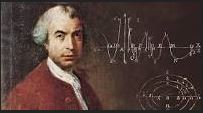
\includegraphics[height=.33\textheight,width=.33\textwidth]{boscovich.jpg}
\end{figure}
\begin{figure}
Karl F. Gauss
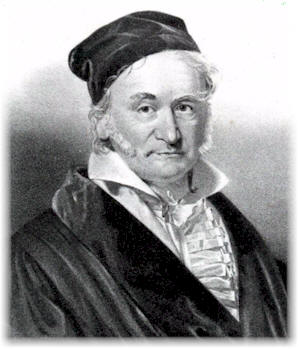
\includegraphics[height=.33\textheight,width=.33\textwidth]{gauss.jpg}
\end{figure}
\onslide<2->{\center --------------------------------------------------------------------}
\end{frame}
\begin{frame}
  \onslide<1->{\frametitle{Least Squares Luminaries} }
\begin{figure}
Peter Swerling
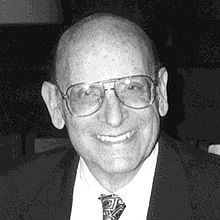
\includegraphics[height=.33\textheight,width=.33\textwidth]{Peter_Swerling.jpg}
\end{figure}
\begin{figure}
Rudolf Kalman
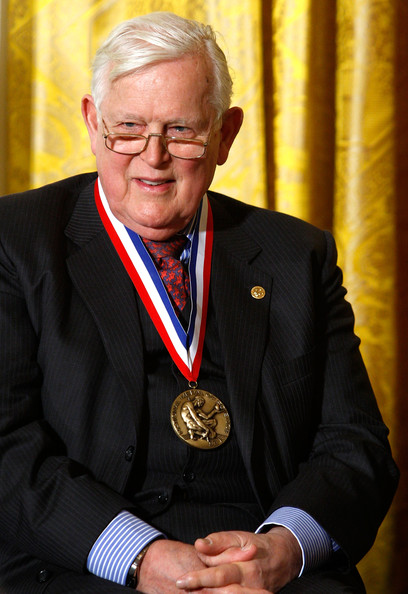
\includegraphics[height=.33\textheight,width=.33\textwidth]{RudolfKalman.jpg}
\end{figure}
\onslide<2->{\center --------------------------------------------------------------------}
\end{frame}

\begin{frame}
\onslide<1->{\frametitle{Kalman Filter Overview}
\framesubtitle{History}}
\begin{itemize}
\onslide<2->{\item Used in early 1960s by Schmidt on Apollo program}
\onslide<3->{\item  Kalman filters are now ubiquitous, especially in navigation}
  \begin{itemize}
     \onslide<4->{
       \item But also in signal processing, econometrics, finance, seismology, weather forecasting, sensor tracking
     }
  \end{itemize}
\end{itemize}
\onslide<5->{\center --------------------------------------------------------------------}
\end{frame}

\begin{frame}
\onslide<1->{\frametitle{Kalman Filter Overview}
\framesubtitle{KF uses in GPS}
}
\begin{itemize}
\onslide<2->{\item All three segments have Kalman filters}
\onslide<3->{\item CS:  ECEST = Ephemeris and Clock Estimator (legacy term), RTGx (JPL's Real-Time GPSY) and NRL's Ensemble Time Filter}
\onslide<4->{\item AEP's ECEST estimates inertial positions and velocities of SVs, solar pressure parameters, 
SV and MS clock error dynamics, and troposphere state at each MS}
\end{itemize}
\onslide<5->{\center --------------------------------------------------------------------}
\end{frame}

\begin{frame}
\onslide<1->{\frametitle{Kalman Filter Overview}
\framesubtitle{KF uses in GPS}
}
\begin{itemize}
\onslide<2->{\item In User Segment receivers, satellite nav software, and offline computations}
\onslide<3->{\item E.g., used in aircraft Operational Flight Programs (OFPs) and Inertial Navigation Systems (INSs) to integrate GPS and other external 
navaids to optimally estimate INS error states }
\onslide<4->{\item 1990s:  Paradigm shift in navigation:\\
  Was: "INS/GPS"\;\;\;\;  Is: "GPS/INS" }
\end{itemize}
\onslide<5->{\center --------------------------------------------------------------------}
\end{frame}


\begin{frame}
\onslide<1->{\frametitle{Kalman Filter Overview}}
\begin{itemize}
\onslide<2->{
	\item State estimation as branch of applied mathematics: 
	Kalman filtering uses techniques and results from many mathematical subjects:\\
linear algebra, differential equations, measure theory, probability, statistics, functional analysis (Hilbert space) 
}
\onslide<3->{
	\item But essentials are very intuitive
}	
	\begin{itemize}
	\onslide<4->{
		\item Can be understood with minimal math background (matrix algebra, calculus, probability and statistics )
	}
	\end{itemize}
\end{itemize}
\onslide<5->{\center --------------------------------------------------------------------}
\end{frame}


\section{Heuristic Introduction}
% \dayonesegone/heuristic_main.tex
\begin{frame}
  \onslide<1->{\frametitle{Part I}
  \framesubtitle{The Basic Kalman Equations\\
  Topics}
  }
 \begin{itemize}
  \onslide<2->{\item Understanding the Equations: Heuristic Introduction}
  \onslide<3->{\item Equation Drilldown:  Taking the Equations Apart}
%  \onslide<4->{\item Differential Equations, Difference Equations and Dynamic Systems}
  \onslide<4->{\item State Space Concepts}
\end{itemize}
\onslide<5->{\center --------------------------------------------------------------------}
\end{frame}

\begin{frame}
\onslide<1->{\frametitle{The Basic Kalman Equations}
\framesubtitle{Understanding the Equations: Heuristic Introduction\\
Subtopics}
}
 \begin{itemize}
 \onslide<2->{\item Recursive Predictor-Corrector Algorithms}
 \onslide<3->{\item Running Averages}
 \onslide<4->{\item Prediction (Extrapolation)}
 \onslide<6->{\item Measurement Update (Correction)}
 \onslide<5->{\item Gain Computation}
\end{itemize}
\onslide<7->{\center --------------------------------------------------------------------}
\end{frame}

\input{\dayonesegone/predict_correct.tex}
\input{\dayonesegone/runavg.tex}
\input{\dayonesegone/extrap.tex}
\input{\dayonesegone/update.tex}
\input{\dayonesegone/gain.tex}
\input{\dayonesegone/exercises.tex}

\section{Equation Drilldown}
% day1_seg2_equations/equation_main.tex


\begin{frame}

\onslide<1->{\frametitle{Part 1}
 \framesubtitle{Equation Drilldown\\Topics}
 }
\begin{itemize}
 
\onslide<1->{\item Understanding the Notation
 }
\onslide<2->{\item Examples
 }
\onslide<3->{\item Exercises
}
\end{itemize}

\end{frame}




% day1_seg1_heuristic/summary.tex

\begin{frame}
  \onslide<1->{\frametitle{Mathematical Formulation of the Problem} 
  \framesubtitle{Kalman Filter Problem Summary}
  }
 \begin{itemize}
  \onslide<2->{   \item Given two models:}
    \begin{itemize}
  	\onslide<3->{\item State Dynamics Model\\ (sometimes called the System or Process Model)}
  	\onslide<4->{\item Measurement Model\\ (sometimes called the Observation Model)}
    \end{itemize}
  \onslide<5->{ \item Find a way to \textbf{optimally} combine our knowledge of the \textbf{predicted state estimate} 
   with our knowledge of the \textbf{actual measurement} to produce an \textbf{updated state estimate}}
  \begin{itemize}
    \onslide<6->{ \item I.e., find the optimal gain with which to weight the measurement residual (difference between actual and predicted measurement) 
	}
    \onslide<7->{ \item Use weighted residual to  increment or update the state estimate} 
	\onslide<8->{ \item Use Kalman gain also to update the estimation uncertainty  
	(estimation error covariance aka "covariance")}
  \end{itemize}
 \end{itemize}
\onslide<9->{\center --------------------------------------------------------------------}

\end{frame}

\begin{frame}
  \onslide<1->{
  \frametitle{Mathematical Formulation of the Problem}
    \framesubtitle{Kalman Filter Problem Summary\\General, Non-Linear, Time-Invariant,
Discrete-Time Formulation }
}
Given:
 \begin{itemize}
   \onslide<2->{ \item State Dynamics Model:  $x(k)=f[x(k-1)] + w(k)$}
   \begin{itemize}
      \onslide<3->{ \item $k$ indicates the time step;  the actual time at that time step is $t_k$, and the time increment is $\Delta t = t_k - t_{k-1}$}
      \onslide<4->{ \item $x(k)$=state vector,$\;\;f$=true dynamics function,$\;\;w(k)$=process noise}
   \end{itemize}
   \onslide<5->{ \item Measurement Model: $z(k)=h[x(k)]+v(k)$}
   \begin{itemize}
      \onslide<6->{ \item $z(k)$=measurement,$\;\;h$=measurement function, $\;\;v(k)$=measurement noise}
   \end{itemize}
  \end{itemize}
  \onslide<7->{ Find:}
 \begin{itemize}
  \onslide<8->{ \item Optimal gain $K(k)$ that allows us to update our state estimate in the following way:\\
     $\hat{x}(k) = f[\hat{x}(k-1)] + K(k)\;[\;z(k)-h(f[\hat{x}(k-1)])\;]$}
  \onslide<9->{ \item (For now, we'll ignore the update of the covariance)}
\end{itemize}
\onslide<10->{\center --------------------------------------------------------------------}
\end{frame}

\begin{frame}
  \onslide<1->{\frametitle{Mathematical Formulation of the Problem} 
  \framesubtitle{Kalman Filter Problem Summary\\
  Limitations}
  }
 \begin{itemize}
  \onslide<2->{ \item Original Kalman filter solution applies only to ...} 
  \begin{itemize}
\onslide<3-> {\item linear systems with linear measurements driven by ...} 	 
\onslide<4-> {\item zero-mean, Gaussian white noise processes (for both process and measurement noise)}
\end{itemize}
\onslide<5->{\item Assume from now on that ...}
  \begin{itemize}
  \onslide<6-> {
    \item  Our vector-valued function $f$ is a linear, vector-valued function, i.e., a matrix $\Phi$
}
  \onslide<7->{
  \item $h$ is also a linear, vector-valued function, i.e. a matrix $H$
}
  \end{itemize}

  \onslide<8->{ \item Thus, the problem is to find a gain matrix $K(k)$ such that} 
  \onslide<9->{\center $\hat{x}(k) = \Phi\hat{x}(k-1) + K(k)\;[\;z(k)-H\Phi\hat{x}(k-1)\;]$  }

\end{itemize}
\onslide<10->{\center --------------------------------------------------------------------}

\end{frame}

\begin{frame}
  \onslide<1->{\frametitle{Mathematical Formulation of the Problem}
  \framesubtitle{Kalman Filter Problem Summary\\ Linear Discrete Formulation\\
 }
}
Given:
\begin{itemize}
  \onslide<2->{\item State Dynamics Model:
  $x(k)=\Phi x(k-1)+w(k)$}
  \onslide<3->{
    \begin{itemize}
		\item $x(k)$=state vector,$\;\;\Phi $=state transition matrix, $\;\;w(k)$=process noise vector
	\end{itemize} }
  \onslide<4->{\item Measurement Model: $z(k)=H x(k)+v(k)$} 
	\begin{itemize}
		 \onslide<5->{\item $z(k)$=measurement vector,$\;\;H$=meas. matrix, $\;\;v(k)$=meas. noise vector}
	\end{itemize}
  \end{itemize}
  \onslide<6->{Find:}
\begin{itemize}
	  \onslide<7->{\item   State estimate in the form\\
 	$\hat{x}(k) = \Phi \hat{x}(k-1) + K(k)[z(k)-H \Phi \hat{x}(k-1)]$ }
\end{itemize}
\onslide<8->{\center --------------------------------------------------------------------}

\end{frame}

\begin{frame}
  \onslide<1->{\frametitle{Mathematical Formulation of the Problem}
\framesubtitle{Kalman Filter Problem Summary \\
Slight Notational Change}
}
\begin{itemize}
  \onslide<2->{  \item The term $\Phi \hat{x}(k-1)$ is the extrapolated state estimate prior to making the measurement update or correction}
  \onslide<3->{  \item To distinguish prior (extrapolated) estimate from updated estimate, we use the following notation:}
   \onslide<4->{  	\[\hat{x}^{-}(k)=\Phi \hat{x}^{+}(k-1)=\text{\textbf{predicted estimate} prior to update}\]}
 \onslide<5->{  \[\hat{x}^{+}(k)=\text{\textbf{updated state estimate}}\] }
  \onslide<6-> {\item Applying $H$ to $\hat{x}^{-}(k)$ yields the \textbf{predicted measurement}}
\end{itemize}
\onslide<7->{\center --------------------------------------------------------------------}

\end{frame}

\begin{frame}
  \onslide<1->{
    \frametitle{Mathematical Formulation of the Problem}
    \framesubtitle{Kalman Filter Problem Solution}
  }
\begin{itemize}
  \onslide<2->{\item Thus, the solution we seek now looks like this:\\}
  \onslide<3->{
    \begin{equation}\label{filtersolution}
       \hat{x}^{+}(k)=\hat{x}^{-}(k)+ K(k)[z(k)-H\hat{x}^{-}(k)]
    \end{equation}
}
\onslide<4-> {
  where $\hat{x}^{-}(k)=\Phi \hat{x}^{+}(k-1) $
}
\onslide<5-> {
  \item This now looks very much like the running average problem!
}
\end{itemize}
\onslide<6->{\center --------------------------------------------------------------------}

\end{frame}



% day1_seg2_equations/notation.tex
\begin{frame}
  \onslide<1->{\frametitle{Understanding Kalman Filter Notation}
\framesubtitle{Drilldown on State Dynamics}
}
 \begin{itemize}
\onslide<2->{ \item State Dynamics Model: $\simplestatedyneq$ }
\onslide<3->{ \item $x(k)$ is the \textit{\textbf{state vector}} with $n$
 elements, written as a column vector:}
\begin{itemize}
\onslide<4->{ \item $x(k)=\state (k)=\statek$}
\end{itemize}
\onslide<5->{ \item The process noise is also a column vector of size $n$:}
	\begin{itemize}
		\onslide<6->{ \item $\procnoise{k}=\procnoisek$}
	\end{itemize}

	\onslide<7->{ \item Some others prefer to make $k$ a subscript;  we choose not to do so, in order to avoid clashes with vector and matrix elements which do by convention use subscripts}

\end{itemize}
\onslide<7->{\center --------------------------------------------------------------------}
\end{frame}

\begin{frame}
  \onslide<1->{\frametitle{Understanding Kalman Filter Notation}
\framesubtitle{Drilldown on State Dynamics}
}
\begin{itemize}
\onslide<2->{ \item Discrete State Dynamics}
\onslide<3->{ \item KF doesn't work for nonlinear dynamics function $f[x(k-1)]$ }
	\begin{itemize}
		\onslide<4->{ \item But nonlinear models can be linearized (more about that later) }
	\end{itemize}
\onslide<5->{ \item Restriction to matrices:  $\simplestatedyneq$}
\onslide<6->{ \item $\stm{k}$ is called the \textbf{state transition matrix}.  It is 
$n\times n$ in size.}
\begin{itemize}
	\onslide<7->{\item If $\Phi$ is derived from a constant-coefficient difference or differential equation, and the time increments $\Delta t$ are constant, there there is no need for the index $k$;  $\Phi$ will then be constant} 
\end{itemize}
\end{itemize}
\onslide<7->{\center --------------------------------------------------------------------}

\end{frame}

\begin{frame}
  \onslide<1->{\frametitle{Understanding Kalman Filter Notation}
\framesubtitle{Drilldown on State Dynamics}
}

\begin{itemize}
\onslide<2->{ \item State Transition Matrix: $\stmeq{k}$}
\onslide<3->{ \item Extrapolates state vector from time step $k-1$ to time step
 $k$ (pulling from past to present)}
\begin{itemize}
	\onslide<4->{\item If $\Delta t = t_k-t_{k-1}$ is constant for all $k$, then we might write $\Phi(\Delta t)$}
\end{itemize}
\onslide<5->{ \item Tells you how the state would evolve \textbf{in the absence of forcing functions}}
\begin{itemize}
	\onslide<6->{ \item Remember: this is still just a model }
	\onslide<7->{ \item  We don't really know
	what the true state is, because the random forcing function (process noise) generates disturbances!}
\end{itemize}

\end{itemize}
\onslide<8->{\center --------------------------------------------------------------------}

\end{frame}

\begin{frame}
  \onslide<1->{\frametitle{Understanding Kalman Filter Notation}
\framesubtitle{Drilldown on State Dynamics}
}

 \begin{itemize}
\onslide<2->{ \item Other factors and terms often play a role in the full state dynamics model}
 \begin{itemize}
\onslide<3->{ \item A matrix $\sdm{k}$ to distribute the Gaussian white noise
 to the states}
\onslide<4->{ \item An additional, deterministic control variable $u(k)$, and
 associated distribution matrix $\Lambda(k)$}
 \onslide<5->{ \item Then the full state dynamics equation would look like this: 
 \[\statedynctrleq\]}
 \end{itemize}
\onslide<6->{ \item In order to focus primarily on the estimation problem, we will generally omit the control variable}
\onslide<7->{ \item Control is obviously an important part of engineering system solutions, so we will consider it occasionally}
\end{itemize}
\onslide<8->{\center --------------------------------------------------------------------}
\end{frame}

\begin{frame}
  \onslide<1->{\frametitle{The Kalman Filter Solution}
\framesubtitle{ State Estimate Extrapolation}
}

\begin{itemize}
\onslide<2->{\item Given an estimate $\stateest{k-1}{+}$ at time $k-1$, we extrapolate it forward in time 
by the state transition matrix:
\begin{equation}\label{stateextrapeq}
\stateextrapeq 
\end{equation}
}
\onslide<3->{\item Q: Why isn't the white noise sequence $w$ included in this extrapolation?}\\  
\onslide<4->{A:  Because the white noise forcing function is a \textbf{zero-mean} process.  
Thus, \textbf{on average}, the equation is homogeneous and we should therefore use the homogeneous solution, i.e., 
the state transition matrix.}
\end{itemize} 
\onslide<5->{\center --------------------------------------------------------------------}
\end{frame}

\begin{frame}
  \onslide<1->{\frametitle{The Kalman Filter Solution}
\framesubtitle{ Covariance Extrapolation}
}

\begin{itemize}
\onslide<2->{\item Q: How certain are we that our solution is right?}\\
\onslide<3->{A: The answer is given by the \textbf{estimation error covariance matrix}, often for brevity just 
called the covariance matrix $P(k)$\onslide<4->{\footnote{\onslide<5->{There are two other covariance matrices involved in KF, but $P$ is often referred to as THE covariance matrix.}}}
}
\onslide<6->{\item Like the state estimate, the covariance matrix is propagated forward in time before being corrected:}
\onslide<7->
{\begin{equation}\label{altcovextrapeq}
\altcovextrapeq
\end{equation}
where $Q(k)$ is a matrix called the \textbf{process noise covariance matrix} }
\onslide<8->{\item $Q(k)$ measures the amount of dispersion in the white noise forcing function $w(k)$}
\onslide<9->{\item Later we'll learn how to define $P(k)$ (at least initially) in terms of the expected error in the estimation $\esterrdef$}
\end{itemize} 
\onslide<10->{\center --------------------------------------------------------------------}
\end{frame}

\begin{frame}
  \onslide<1->{\frametitle{The Kalman Filter Solution}
\framesubtitle{ Covariance Extrapolation}
}
\begin{itemize}
\onslide<2->{\item What does Eq. \eqref{altcovextrapeq} really mean?
  \[ \altcovextrapeq \]
}
\onslide<3->{\item The term $\stm{k}\covmat{k-1}{+}\stm{k}\trans$ represents the effect that the state dynamics 
has on the estimation error covariance}
\begin{itemize}
\onslide<4->{\item P(k) is a positive definite matrix and $\Phi $ tends to increase its norm }
\end{itemize}
\onslide<5->{\item The other term $Q(k)$ represents the increased uncertainty added at each step due to 
the process noise inherent in the system (like all covariance matrices, it is also positive definite) }
\end{itemize} 
\onslide<6->{\center --------------------------------------------------------------------}
\end{frame}



\begin{frame}
  \onslide<1->{\frametitle{Examples}}
\begin{itemize}
 \onslide<2->{\item The Examples present three different models:}
 \begin{itemize}
 \onslide<3->{\item Resistor Revisited (but using a Kalman filter instead of a running average)}
 \onslide<4->{\item Constant Velocity Motion (non-accelerated motion)}
 \onslide<5->{\item Damped Harmonic Oscillator}
\end{itemize}
 \onslide<6->{\item Types of Plots produced by the simulations} 
\end{itemize} 
\onslide<7->{\center --------------------------------------------------------------------}
\end{frame}

\begin{frame}
  \onslide<1->{\frametitle{Overview of the Examples}}
\begin{itemize}
  \onslide<2->{\item Discrete-time systems}
  \onslide<3->{\item Gradually increasing complexity:  }
  \begin{itemize}
    \onslide<4->{\item Resistor: 1 state, \textbf{static} (constant dynamics)  }
    \onslide<5->{\item Constant Velocity Motion:  2 states, with one state \textbf{dynamic} and one \textbf{static} }
    \onslide<6->{\item Damped Harmonic Oscillator:  2 states, with \textbf{both states dynamic}  }
  \end{itemize}
\end{itemize}
\onslide<7->{\center --------------------------------------------------------------------}
\end{frame}

\begin{frame}
  \onslide<1->{
  \frametitle{ The MATLAB/Python files:\\ 
		\texttt{kf\_resistor\_demo,constant\_velocity, damposc} in both .m and .py versions}
}
\begin{itemize}
  \onslide<2->{\item File located here: matlab/python \\
    \url{https://github.com/musicarroll/kalman_course/src }
	}
  \onslide<3->{\item Download these scripts and play with them!  }
  \begin{itemize}
	\onslide<4->{\item Modify the initial conditions, number of samples  }
  	\onslide<5->{\item Modify the $R$ and $Q$ noise parameters  }
	\onslide<6->{\item Observe how the plots change }
  \end{itemize}
  \onslide<7->{ \item If you want to share your mods to the programs, upload them to the 
  student\_contrib folder on github}
  \onslide<8-> {\item Please add a suffix (such as your YouTube ID) to filename:  \\
  E.g. damposc\_joeuser.py
  }
\end{itemize}
\onslide<9->{\center --------------------------------------------------------------------}
\end{frame}


\begin{frame}
  \onslide<1->{\frametitle{Types of Plots}}
\begin{itemize}
  \onslide<2->{\item Truth/Measurement/Estimation (TME) plots}
  \begin{itemize}
	\onslide<3->{\item Time series plots of ground truth model, measurements, and state estimations}
  \end{itemize}
  \onslide<4->{\item Kalman Sawtooth plots}
  \begin{itemize}
    \onslide<5->{\item Specialized plots for simultaneously assessing the growth and reduction in estimation uncertainty }
  \end{itemize}
\end{itemize}
\onslide<6->{\center --------------------------------------------------------------------}
\end{frame}

\begin{frame}
  \onslide<1->{
	\frametitle{TME Plots} 
	\framesubtitle{Truth, Measurement, Estimation Plots}
}
  \onslide<2->{
\begin{figure}
  \includegraphics[width=0.95\textwidth,height=7cm]{\dayonesegtwo/damposc_conservative.png}
\end{figure}   
}
\onslide<3->{\center --------------------------------------------------------------------}
\end{frame}


\begin{frame}
  \onslide<1->{\frametitle{Kalman Sawtooth Plots}}
  \begin{itemize}
   \onslide<2->{\item Interleave pre- and post-update elements of $P$ over a run
   }
   \onslide<3->{\item Show growth over time in uncertainty (upticks) and 
   then immediate reduction (no time lapse!) in uncertainty (downticks) after measurement updates 
}
\onslide<4->{   
\begin{figure}
  \includegraphics[width=0.75\textwidth,height=5cm]{\dayonesegtwo/kf_resistor_variance_w_process_noise.png}
\end{figure}
}
\end{itemize}
\onslide<5->{\center --------------------------------------------------------------------}
\end{frame}


%\input{\dayonesegtwo/03_01_resistor.tex}
%\input{\dayonesegtwo/03_02_constant_velocity.tex}
%\input{\dayonesegtwo/03_03_damposc.tex}





% day1_seg2_equations/exercises.tex

\begin{frame}

  \onslide<1->{\frametitle{Exercises
}}
\begin{enumerate}
  \onslide<2->{\item Work through the resistor example by hand using 
$\hat{x}_0=100\Omega$, $\sigma=0.1$, and $P_0=0$.  Start the recursive loop 
with the gain equation first.  Run through the loop three times.}

  \onslide<3->{
\item Draw a rough plot of the error covariance, plotting both the extrapolated and 
updated covariance for any give $k$ at the same time.  (This will yield the classic 
Kalman sawtooth pattern.)
  Similarly, draw a rough plot of the state estimates.}

\setcounter{exercisecounter}{\value{enumi}}
\end{enumerate}
\end{frame}


\begin{frame}


  \onslide<1->{\frametitle{Exercises
}}
\begin{enumerate}
\setcounter{enumi}{\value{exercisecounter}}
  \onslide<2->{\item Calculate the Kalman gain of the non-accelerated motion example.  Hint:  It looks a lot like the 
gain for the damped harmonic oscillator.}
  \onslide<3->{\item Write out the state update equation for the damped harmonic oscillator, 
using the Kalman gain derived in the example.

}
  \onslide<4->{\item Write out the covariance update 
equation for the damped harmonic oscillator, using the Kalman gain dervied in the 
example.
 }
\end{enumerate}
\end{frame}


%\section{Dynamic Systems}
%% day1_seg2_diff_eq/state_space_main.tex
\begin{frame}
\textbf{Segment 3\\
Differential Equations and Difference Equations\\
Topics}
 \begin{itemize}
   \item Input-Output Representation
   \item Differential Equations and Difference Equations
\end{itemize}
\end{frame}
% day1_seg3_state_space/input_output.tex

\begin{frame}
Input-Output Representation
 
\begin{itemize}
 
\item Black box approach:  $y(t)=f(u(t),t)$\\

 
\begin{figure}
   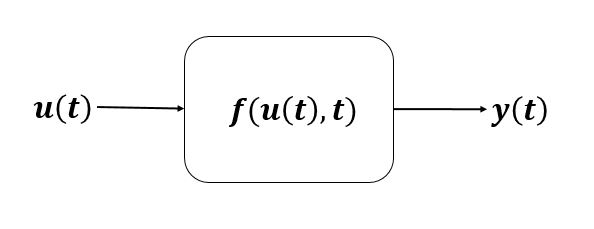
\includegraphics[width=0.85\textwidth]{day1_seg3_diff_eq/input_output.jpg}

 
\end{figure}
\item Output represents the resultant behavior of the dynamic system as a function 
of the input (and possibly time).
 
\item Output is often one primary scalar variable of interest like position.

\end{itemize}

\end{frame}



\begin{frame}
Input-Output Representation
 
\begin{itemize}
 
\item Note that output is not necessarily the same thing as the observation or measurement.
 
\item Observation or measurement is often related directly to the output through a matrix coupling.
 
\item In state space representation, the output is often eliminated in favor of the state vector, and 
the measurement is given as a function of the state vector directly.

\end{itemize}

\end{frame}



\begin{frame}
Input-Output Representation
 
\begin{itemize}
 
\item The derivatives of position and how they relate to the forcing function yields a single differential equation.
 
\item We'll see later how an $n^\text{th}$-order, scalar differential equation is related to a 
vector state space model. 



\begin{itemize}
  \item In fact, the state vector be comprised of the values of the initial conditions for the differential 
equation at any particular time.
\end{itemize}


\end{itemize}

\end{frame}

% day1_seg3_diff_eq/diff_eq.tex

\begin{frame}
Differential Equations and Difference Equations
\\
A Mini Refresher Course 
\begin{itemize}
 
\item Ordinary Differential Operators
 
\item Ordinary Differential Equations
 
\item Difference Equations

\end{itemize}

\end{frame}


% orddiffops.tex

\begin{frame}
Ordinary Differential Operators: Vectors and Functions

\begin{itemize}
  \item Vectors are functions and functions are vectors
  
\item A vector $\begin{bmatrix}x_1\\x_2\\x_3\end{bmatrix}$ in 3-space is really a 
function $x:\set{1,2,3}\rightarrow \Real$
  
\item We just write them differently than functions, i.e., instead of $x(i)$ 
we write $x_i$. 

\end{itemize} 

\end{frame}


\begin{frame}
Ordinary Differential Operators: Vectors and Functions
 
\begin{itemize}
  
\item And since the domain $\set{1,2,3}$ of the function $x$ is so small, we can 
exhibit all values of $x$ explicitly in one fell swoop, i.e., 
as $\begin{bmatrix}x_1\\x_2\\x_3\end{bmatrix}$
  
\item But, by the same token, ordinary real functions $f:\Real\rightarrow\Real$ are 
vectors
  
\item They just have so many components that we can't exhibit them all at once

\end{itemize} 

\end{frame}


\begin{frame}
Ordinary Differential Operators: Vectors and Functions

\begin{itemize}
  
\item We can add vectors by adding their components: $z=x+y$ if and only if 
$z_i=x_i+y_i$ for each index $i$
  
\item By the same token, we can add functions componentwise:
  $h=f+g$ if and only 
if $h(t)=f(t)+g(t)$ for all $t$ in the domain
  
\item Componentwise multiplication of functions can also be defined 
(although this does not come up as often for ordinary vectors):  $h=f\cdot g$ if 
and only if $h(t)=f(t)\cdot g(t)$ for all $t$ in the domain

\end{itemize} 

\end{frame}



\begin{frame}
Ordinary Differential Operators: Vectors and Functions

\begin{itemize}
  
\item Finally, we can multiply functions by scalars, just like we do for vectors:  
$g=a\cdot f$ if and only if $g(t)=a\cdot f(t)$ for all $t\in\Real$.
  
\item The upshot of all this is that the set of all real functions is a vector space!
  
\item But we are really more interested in a subspace of this vector space, i.e., we really want to 
restrict our attention to the set of all \textbf{differentiable} functions on some closed interval.

\end{itemize} 

\end{frame}


\begin{frame}
Ordinary Differential Operators: Differentiable Functions

\begin{itemize}
  
\item Let $I=[a,b]$ be any closed interval of the real line
  
\item Consider the set $\Real^I=\set{f:I\rightarrow \Real}$ of all functions mapping $I=[a,b]$ into the real numbers
  
\item Then, as we have just pointed out, $\Real^I$ is a vector space over the reals

\end{itemize} 

\end{frame}



\begin{frame}
Ordinary Differential Operators
 
\begin{itemize}
  
\item We define the \textbf{\textit{derivative}} of a function $f$ at the point $t\in [a,b]$ as the 
limit as $s\rightarrow
 t$ of the difference quotient,
 \[\frac{f(s)-f(t)}{s-t},\]
assuming this limit exists.
  
\item Note that not all functions have derivatives!
  
\item Those that do have a derivative defined at every point of $I$ we call \textbf{\textit{differentiable}} on $I$.

\end{itemize} 

\end{frame}



\begin{frame}
Ordinary Differential Operators
 
\begin{itemize}
  
\item This operation turns out to be a linear operator on the vector space of functions that are differentiable 
on $I=[a,b]$.
  
\item In fact, we want to consider those functions that can be differentiated as many times as we like
  
\item Thus, we consider the space of infinitely differentiable, real-valued functions defined on the 
closed real interval $[a,b]$: $C^\infty[a,b]$
\end{itemize}

\end{frame}


% orddiffeqs.tex

\begin{frame}
Ordinary Differential Operators
 
\begin{itemize}
 
\item The operation of taking the derivative will enable us to develop deterministic differential
 equations.
 
\item Later we will define derivatives of stochastic processes in order to introduce and solve stochastic 
differential equations.  You cannot always take the derivative (or even integrate) a random process -- 
and sometimes not even the sample functions of a random process -- in the ordinary sense.

\end{itemize}

\end{frame}


% orddiffeqs.tex

\begin{frame}
Ordinary Differential Operators
 
\begin{itemize}
 
\item Since the derivatives of all orders are assumed to exist
 for all functions $f\in C^\infty[a,b]$, the 
limit of the
 difference quotient always exists for such functions.
 
\item Thus, we assign to each $f$ a new function $Df$ given by

\begin{equation}\label{deriv}
  [Df](t) = \lim_{s\rightarrow t}\frac{f(s)-f(t)}{s-t}
\end{equation}
 
\item This assignment defines a transformation
 \[D:C^\infty[a,b]\rightarrow C^\infty[a,b]\]
  that is a linear operator.

\end{itemize}

\end{frame}


\begin{frame}
Ordinary Differential Operators
 
\begin{itemize}
    
\item $D$ is linear: $D[af+bg]=a[Df] + b[Dg]$
    
\item Sometimes we get lax and simply write $Df(t)$ instead of $[Df](t)$.  However, keep in mind that $Df(t)$ 
says "Differentiate $f$ and then evaluate the resulting function at the point $t$."
    
\item $D$ obeys all the usual rules of differential calculus such as the product rule and the chain rule:

\[D(fg)=[Df]g+f[Dg]\]
\[D(f\circ g) = [Df]\circ g \cdot Dg\]
 
\end{itemize}

\end{frame}


\begin{frame}
Ordinary Differential Operators: Examples
 
\begin{itemize}
  
\item If $\id$ is the identity function, i.e., $\id(t)=t$, then
 $D\id=1$. (You probably know this 
as $\frac{dt}{dt}=1$; Note that 1 is the function whose value at every $t$ is 1.)
  
\item Using the product rule, we have, for example,

\begin{align*}
D\id^2 &= D\left[\id \cdot \id \right]\\
&= D\id \cdot \id + \id \cdot D\id\\
&= 1 \cdot \id + \id \cdot 1\\
&= \id + \id\\
&= 2\id
\end{align*}

(In more familiar notation this is just $\frac{dt^2}{dt}=2t$.)
 
\end{itemize}

\end{frame}


% orddiffeqs.tex

\begin{frame}
Ordinary Differential Operators
 
\begin{itemize}

 \item Note that we sometimes write $d/dt$ or $\frac{d}{dt}$ for
 the operator $D$ when we want to emphasize 
the independent
 variable $t$.  Or, instead of $\frac{dy}{dt}$ we write simply $\dot{y}$.
 
\item However, that is really unnecessary, adds no new information, and is just extra
 baggage.
 
\item Nevertheless, we shall do it sometimes because it may be more familiar.

\end{itemize}

\end{frame}


% orddiffeqs.tex

\begin{frame}
Ordinary Differential Operators
 
\begin{itemize}
 
\item Since there is really only one generating operator $D$ that we are interested in here,
 
we are less interested in multiplication than we are in function
 composition or iteration of this operator. 
For instance,
 $D^2f=[D\circ D](f) = D(Df)$.
 
\item By induction we have $D^n=\underbrace{D\circ\cdots \circ D}_n$.
 
\item Just as real-valued functions inherit algebraic operations from those of their range
 spaces, 
so too do differential operators:
 \[\left[aD^m+bD^n\right](f)=a(D^mf)+b(D^nf)\]

\end{itemize}

\end{frame}


% orddiffeqs.tex

\begin{frame}
Ordinary Differential Operators
 
\begin{itemize}
 
\item We can therefore generate polynomials in $D$:
 \[p(D)=a_nD^n+\cdots +a_1D+a_oI,\]
 
where $I$ is the identity operator on $C^\infty[a,b]$.  We
 usually just drop the identity operator, 
since it amounts to multiplying by 1.
 
\item Such polynomials in $D$ are still linear operators.
 
\item Thus, we have rediscovered the group
 ring $\Real(\Diff)$, where $\Diff$ in this case is the 
infinite cyclic
 group generated by the differential operator $D$.  We'll call
 this group ring 
 
the \textit{\textbf{polynomial ring of differential operators}}.

\end{itemize}

\end{frame}


\begin{frame}
Ordinary Differential Equations
 \begin{itemize}
 \item With polynomials of differential operators we can now
 define ordinary differential equations.
 \item An equation of the form
 \[p(D)f=q(D)g\]
 where  $f,g\in \Cinf$ and $p(D),q(D)\in \Real(\Diff)$,
 is called an ordinary differential equation with constant
 coefficients.
\end{itemize}
\end{frame}
% orddiffeqs.tex
\begin{frame}
Ordinary Differential Equations
 \begin{itemize}
 \item It is probably more familiar if we use $y$
 instead of $f$ and $u$ instead of $g$, and if we show the
 independent variable, say t, explicitly:
 \[a_n\frac{d^ny}{dt^n}+\cdots +a_1\frac{dy}{dt}+a_0y =
 b_m\frac{d^mu}{dt^m}+\cdots + b_1\frac{du}{dt}+b_0u\]
 or
\begin{equation}\label{diffeq}
\diffeq
\end{equation}
 \item For our purposes, the function $u=u(t)$ is called the \textit{\textbf{input}},
 while the function $y=y(t)$ is called the \textit{\textbf{output}}.  The
 independent variable $t$ is thought of as time.
\end{itemize}
\end{frame}
\begin{frame}
Ordinary Differential Equations
 \begin{itemize}
 \item In \eqref{diffeq}, $u$ is ordinarily assumed to be known or given,
 while $y$ is unknown and sought.
 \item Any function $y$
 satisfying \eqref{diffeq} is called a solution of the
 differential equation.
 \item A differential equation such as \eqref{diffeq} is called
 \textit{\textbf{homogeneous}} when the input function $u$ is identically zero
 for all $t\in[a,b]$.
\end{itemize}
\end{frame}
\begin{frame}
Ordinary Differential Equations
 \begin{itemize}
 \item Thus far we have only dealt with linear differential equations
 with constant coefficients.
 \item We could allow the coefficients to be time-dependent
 functions.  However, for most of our applications, this will not
 be necessary.
\end{itemize}
\end{frame}
% orddiffeqs.tex
\begin{frame}
Ordinary Differential Equations: Examples
 \begin{itemize}
 \item From physics we have Hooke's law: the restoring force of a
 spring is proportional to the distance stretched:  $-ky = m\frac{d^2y}{dt^2}$.
 \item This is just an application of Newton's $F=ma$, where $a$
 is the acceleration: $a=d^2y/dt^2$.
 \item Rewriting this in the form of \eqref{diffeq} we have
 \[m\frac{d^2y}{dt^2}+ky=0\]
 \item Therefore, this is a homogeneous equation of order 2.
\end{itemize}
\end{frame}
% orddiffeqs.tex
\begin{frame}
Ordinary Differential Equations
 \begin{itemize}
 \item We have used $y$ rather than $x$ as in most physics books,
 because we want to be consistent with \eqref{diffeq}.
 \item It is common to rewrite such equations so that the leading
 coefficient is 1.  Thus we have:
 \[\frac{d^2y}{dt^2}+\frac{k}{m}y=0.\]
 \item It is easily verified that $\sin\omega_0 t$, where
 $\omega_0=\sqrt{\frac{k}{m}}$, satisfies this differential equation.
\end{itemize}
\end{frame}
\begin{frame}
Ordinary Differential Equations
 \begin{itemize}
 \item Equation \eqref{diffeq}
 \[\diffeq\]
 is called
 \textit{\textbf{time-invariant}}, because the coefficients are
 constant and also because the independent variable $t$ does not
 appear explicitly in the equation.
 \item Note that \eqref{diffeq} is linear in terms of both the
 input and the output, because the polynomial differential
 operator on each side of the equation is a linear operator.
\end{itemize}
\end{frame}
\begin{frame}
Ordinary Differential Equations
 \begin{itemize}
 \item This double linearity means, on the one hand, that the output $y$ due to several inputs acting
 at the same time is equal to the sum of the outputs due to each
 input acting alone.
 \item On the other hand, it also means that if $y_1$ and $y_2$
 are both solutions to the homogeneous version of \eqref{diffeq},
 then so is $c_1y_1+c_2y_2$ where $c_1$ and $c_2$ are any real
 constants.
 \item A maximal set of $n$ such solutions to the homogeneous
 equation that are also linearly independent (as vectors) is
 called a \textit{\textbf{fundamental set}}.
\end{itemize}
\end{frame}
\begin{frame}
Ordinary Differential Equations
 \begin{itemize}
 \item You can find a fundamental set by solving the
 \textit{\textbf{characteristic equation}} associated with the differential equation.  This equation is
 nothing other than the original polynomial equation in $D$, but
 with $D$ replaced by an unknown such as $z$.
 \item Thus, the characteristic equation for \eqref{diffeq} is
 \[a_nz^n+\cdots + a_1z + a_0=0\]
 \item We use $z$ because the roots of this equation are in
 general complex (thanks, once again, to Dr. Gauss).
\end{itemize}
\end{frame}
\begin{frame}
Ordinary Differential Equations
 \begin{itemize}
 \item In solving the characteristic equation, two cases emerge:
 \begin{enumerate}
 \item The roots of the characteristic equation are all distinct.
 \item Some roots are repeated, i.e., each root $r_i$ has
 multiplicity $n_i$.
 \end{enumerate}
\end{itemize}
\end{frame}
\begin{frame}
Ordinary Differential Equations
 \begin{itemize}
 \item In case 1, a fundamental set is easily constructed:
 \[y_1(t)=\exp(r_1t),\ldots,y_n(t)=\exp(r_nt) \]
 where the $r_i$ are the distinct roots.
 \item In case 2, each root $r_i$ of multiplicity $n_i$ contributes
 $n_i$ functions to the fundamental set:
 \[y_{i1}(t)=\exp(r_it),y_{i2}(t)=t\exp(r_it),\ldots,y_{in_i}(t)=t^{n_i-1}\exp(r_it) \]
\end{itemize}
\end{frame}
\begin{frame}
Ordinary Differential Equations
 \begin{itemize}
 \item To fully solve the differential equation, the initial
 conditions need to be taken into account.
 \item These are the values of the function and its first $n-1$
 derivatives at the start of the time interval.
 \item We will specialize our interval $[a,b]$ to the case in which $a=0$
 and $b=T$, some unspecified time in the future.
\end{itemize}
\end{frame}
\begin{frame}
Ordinary Differential Equations
 \begin{itemize}
 \item The \textit{\textbf{free response}} is the solution to the homogeneous
 equation in which the initial conditions are specified but the input is zero, i.e., there is no forcing function.:
\begin{equation}\label{initcond}
  y(0),Dy(0),\ldots,D^{n-1}y(0)
\end{equation}
 \item The \textit{\textbf{forced response}} reverses this situation; it allows the
 input function to be non-zero, but it requires all the initial
 conditions in \eqref{initcond} to be zero.
 \item The \textit{\textbf{total response}} is the sum of the free and forced
 responses.
\end{itemize}
\end{frame}
\begin{frame}
Ordinary Differential Equations: Example of Free, Forced and Total
Responses
 \begin{itemize}
 \item Consider $D^2y+3Dy-1y=u$ with initial conditions:
 $y(0)=1,Dy(0)=-1$.
 \item The roots (found using Matlab's roots function) are $r_1=-3.3028$ and $r_2=0.3028$, and they are
 distinct.
 \item Therefore, a fundamental set is
 $\set{\exp(-3.3028t),\exp(0.3028t)}$.
\end{itemize}
\end{frame}
\begin{frame}
Ordinary Differential Equations: Example of Free, Forced and Total
Responses
 \begin{itemize}
 \item With the fundamental set and the initial conditions we can
 form a set of $n$ linear equations in $n$ unknowns (here, $n=2$):
\begin{align*}
  c_1y_1(0)+c_2y_2(0) & =y(0) \\
  c_1Dy_1(0)+c_2Dy_2(0) & =Dy(0)
\end{align*}
or
\begin{align*}
  1\cdot c_1+1\cdot c_2 & =0 \\
  -3.3028\cdot c_1+0.3028\cdot c_2 & =-1
\end{align*}
\end{itemize}
\end{frame}
\begin{frame}
Ordinary Differential Equations
 \begin{itemize}
 \item The previous linear system is of the form $Ax=b$.  Using
 Matlab's matrix division operator $\backslash$, the solution is
 $x = A\backslash b$ or
\begin{align*}
  c_1 & =    0.2773 \\
  c_2 & =   -0.2773
\end{align*}
%\item We can easily verify that
%$y(t)=0.2773\exp(-3.3028t)-0.2773\exp(0.3028t)$ is indeed the free
%response by plugging and chugging
%\begin{align*}
%  D^2y+3Dy-1y & =D^2[0.2773\exp(-3.3028t)-0.2773\exp(0.3028t)]\\
%   & \quad +3D[0.2773\exp(-3.3028t)-0.2773\exp(0.3028t)]\\
%   & \quad -1[0.2773\exp(-3.3028t)-0.2773\exp(0.3028t)] \\
%   & = 0.2773\cdot 3.3028^2\exp(-3.3028t)\\
%   & \quad -0.2773\cdot 0.3028^2\exp(0.3028t)\\
%   & \quad +3\cdot 0.2773\cdot (-3.3028)\exp(-3.3028t)\\
%   & \quad -3\cdot 0.2773\cdot 0.3028\exp(0.3028t)\\
%   & \quad -0.2773\exp(-3.3028t)+0.2773\exp(0.3028t)
%\end{align*}
\end{itemize}
\end{frame}
\begin{frame}
Ordinary Differential Equations
 \begin{itemize}
 \item The total response can also be decomposed into transient
 and steady state responses
 \item The \textit{\textbf{transient}} response is that part of the total response
 that decays to 0 as $t\rightarrow \infty$.
 \item The \textit{\textbf{steady state response}} is the difference between the
 total response and the transient response.
\end{itemize}
\end{frame}
\input{day1_seg3_diff_eq/lti.tex}


% difference_eq.tex
\begin{frame}
Ordinary Difference Equations
\begin{itemize}
  \item Auto-Regressive Moving Average (ARMA)
  \item $n^{\text{th}}$ derivative corresponds to $n$-step advance:
\end{itemize} 
\begin{equation}\label{armaeq}
\armaeq
\end{equation}
\end{frame}
\begin{frame}
Ordinary Difference Equations
\begin{itemize}
  \item The left side of Eq. \eqref{armaeq} is the Auto-Regressive part
  \item The right side of Eq. \eqref{armaeq} is the Moving Average part
  \item Hence, ARMA
\end{itemize} 
\end{frame}
\begin{frame}
Ordinary Difference Equations: Example
\begin{itemize}
  \item Let $n=3$, $m=2$ and consider the difference equation:
\begin{align*}
-3y(k+3)+1.5y(k+2)\\
 +7y(k+1)-3.2y(k)\\
&=23u(k+2)-5u(k+1)+0.5u(k)
\end{align*}
\end{itemize} 
\end{frame}



% \input{day1_seg3_state_space/stoch_diff_eq.tex}
%% day1_seg3_state_space/exercises.tex
\begin{frame}
Exercises
 \begin{itemize}
 \item
 \item
 \item
\end{itemize}
\end{frame}


\section{State Space Concepts}
\begin{frame}
  \onslide<1->{\frametitle{State Space Concepts}
\framesubtitle{Topics} 
}
\begin{itemize}
  \onslide<2->{
\item  Dynamic Systems: Differential Equations and the Concept of State Space
}
  \onslide<3->{
\item  Diagrams and State Space 
}
  \onslide<4->{
\item   State Transition Matrix
}
\end{itemize}
\onslide<5->{\center --------------------------------------------------------------------}
\end{frame}

% \input{day1_seg3_state_space/stoch_diff_eq.tex}


\begin{frame}
  \onslide<1->{\frametitle{Dynamic Systems} 
  \framesubtitle{The Concept of State Space}
}
  
\begin{itemize}
  \onslide<2->{
\item Time-dependent behavior of physical systems often
 modeled analytically by \emph{differential equations}
}
  \onslide<3->{
\item  Called \textit{\textbf{dynamic systems}} or
 \textit{\textbf{dynamical systems}}
}
  \onslide<4->{
	\item  Smooth processes:  described by continuous, differentiable functions of time
}
\end{itemize}
\onslide<5->{\center --------------------------------------------------------------------}
\end{frame}


\begin{frame}
	\onslide<1->{\frametitle{Dynamic Systems}
	\framesubtitle{Newton's Laws of Motion} }
	\begin{itemize}
		\onslide<2->{
			\item Newton's first two laws specify what happens when a body is subjected to a force.   
		}
		\onslide<3->{
			\item Whenever a net force acts on a body, the body's velocity will change, i.e., it will accelerate or decelerate  (First Law)
		}
		\onslide<4->{
			\item For a constant net force, the motion will be such that the product of the body's mass and its acceleration will be invariant (i.e., the same for all bodies) (Second Law)
		}
		\begin{itemize}
		\onslide<5->{
			\item Under the same constant force, large bodies will exhibit a small acceleration, while small bodies will exhibit a larger acceleration
		}
		\end{itemize}
	\end{itemize}
	\onslide<6->{\center --------------------------------------------------------------------}
\end{frame}



\begin{frame}
  \onslide<1->{\frametitle{Dynamic Systems}
  \framesubtitle{Newton's Laws of Motion}
 }
\begin{itemize}
  \onslide<2->{
\item In Newton's Second law $F=ma$, the resultant force $F$ acts on the mass $m$ to produce an acceleration:
\begin{equation}
F=ma=m\dot{v}=m\deriv{v}{t}=m\secondderiv{y}{t}=m\ddot{y}
\end{equation}  
}
  \onslide<3->{
	\item Since acceleration is the second derivative of position, Newton's Second law often leads to \textbf{second order} differential equations (whenever the acceleration is constant, i.e., $\dot{a}=0$); the solution $y(t)$ is considered to be the \textbf{output} of the dynamical system   
}
  \onslide<4->{
	\item The resultant force is the vector sum of all forces acting on the body, both \textbf{internal} coupling forces and \textbf{external} input forces  
}
\end{itemize}
\onslide<5->{\center --------------------------------------------------------------------}
\end{frame}

\begin{frame}
	\onslide<1->{\frametitle{Dynamic Systems} 
	\framesubtitle{A Note on Notation}
	}
	\begin{itemize}
		\onslide<2->{ \item In pure mathematics, one often sees $y$ as a function of $x$:  $y=f(x)$.  
		}
		\onslide<3->{
			\item  However, in engineering work, the variable $x$ is often reserved to be used as the (vector) state variable.
		}
		\onslide<4->{
			\item Moreover, in dynamic systems, $y$ is generally considered to be a function of time $t$.  Hence our use of symbols such as \\ $y(t)$, $\dfrac{dy}{dt}$, $\Dopnth{n}{t}{y}$, $\dot{y}$, $\ddot{y}$, etc.
		}
		\onslide<5->{
			\item  In physics, the variable $r=r(t)$ is often used to stand for displacement (position), with 3d coordinates of $x,y,z$.
		}
		\onslide<6->{
			\item In these slides we are mostly using standard engineering notation.
		}
		\onslide<7->{
			\item It is also common in engineering notation to use $u=u(t)$ as the symbol for external input -- or control -- function.
		}
	\end{itemize}
	\onslide<8->{\center --------------------------------------------------------------------}
\end{frame}

\begin{frame}
  \onslide<1->{\frametitle{Dynamic Systems}
	\framesubtitle{Internal and External Forces}  
}
\begin{itemize}
  \onslide<2->{ \item Which forces are considered internal and which external depends on how the system boundary is drawn  
}
  \onslide<3->{
\item  Simple harmonic oscillator has one internal force determining system behavior: $F=-ky$, because the spring itself is often considered a (massless) part of the system  \\(more complicated oscillators may also include internal frictional and/or external driving forces)
}
\onslide<4->{
	\item Spring forces (e.g., Hooke's law, where $F=-ky$) are often considered to be \textbf{internal} to system
}
  \onslide<5->{
\item  External forces (e.g., constant or time-dependent forcing functions) may also be present, e.g.:
 \[\frac{d^2y}{dt^2}+\frac{k}{m}y=\dfrac{1}{m}\sin\omega t\]
}
\onslide<6->{
	\item Internal forces are generally not viewed as \textbf{inputs}
}
\end{itemize}
\onslide<7->{\center --------------------------------------------------------------------}
\end{frame}

\begin{frame}
  \onslide<1->{\frametitle{Dynamic Systems} 
	\framesubtitle{Second-Order Mechanical Systems}
}
\begin{itemize}
  \onslide<2->{
\item Most general second-order equation for a mechanical
 system of this type (according to Newton's law) is:
\begin{equation}\label{second ord}
 \ddot{y} =\frac{1}{m}F(y,\dot{y},t)
\end{equation}  
}
  \onslide<3->{
\item If $F(y,\dot{y},t)$ can be expressed 
as sum of $F_1(y,\dot{y})$ and $F_2(t)$, then
 we can write this in input-output form:
  \[\ddot{y}-\frac{1}{m}F_1(y,\dot{y})=\frac{1}{m}F_2(t)\]
}
  \onslide<4->{
	\item Note that the left hand side is a function only of $y$ and its derivatives, while the right hand side is a function of time only.
}
\end{itemize}
\onslide<5->{\center --------------------------------------------------------------------}
\end{frame}



\begin{frame}
	\onslide<1->{\frametitle{The Concept of State} }
	\begin{itemize}
		\onslide<2->{
			\item Concept of state involves in some sense the instantaneous internal arrangement and relationships of a system's components
		}
		\onslide<3->{
			\item In practical  situations, the state variables may represent attributes of the  system that we wish to know something about 
		}
		\onslide<4->{
			\item Also intuitively, state variables are usually naturally coupled in some sense; 
			this is obvious when they are derived from a single differential equation in which all quantities are derivatives 
			of a single variable (the output variable)  
		}
	\end{itemize}
	\onslide<5->{\center --------------------------------------------------------------------}
\end{frame}


\begin{frame}
  \onslide<1->{\frametitle{The Concept of State} 
	\framesubtitle{State as Initial Conditions}  
}
\begin{itemize}
  \onslide<2->{
	\item \footnotesize{"How is a dynamic system (linear or nonlinear) described?
		The fundamental concept is the notion of the state.  By this is meant, intuitively, some quantitative information 
		(a set of numbers, a function, etc.) which is the least amount of data one has to know about the past behavior of 
		the system in order to predict its future behavior."\\
		Rudolf Kalman, in seminal paper (1960)}
}
  \onslide<3->{
\item To determine behavior of deterministic system at any future time requires knowledge of two things:
\begin{enumerate}
\item Equations governing the system dynamics (usually differential of difference equations)
\item Initial conditions
\end{enumerate}  
}
  \onslide<4->{
\item But initial conditions for an $n^{\text{th}}$-order continuous dynamic system are simply values of first $n$ derivatives at initial time (the Identity operator can be considered the 0th order derivative)
}
  \onslide<5->{
	\item The $n^{\text{th}}$-order derivative is given essentially by the differential equation itself
}

\end{itemize}
\onslide<5->{\center --------------------------------------------------------------------}
\end{frame}

\begin{frame}
  \onslide<1->{\frametitle{The Concept of State} }
\begin{itemize}
  \onslide<2->{
\item At any point in time, we can think of instantaneous values of first $n$ derivatives as initial conditions for all future dynamic evolution  
}
  \onslide<3->{
\item The first $n$ derivatives are the $0^\text{th},1^\text{st},\ldots,(n-1)^\text{st}$ derivatives of the output function $y$
}
  \onslide<4->{
	\item These values capture the "state" of the dynamic system at any time after the time of the initial conditions  
}
\end{itemize}
\onslide<4->{\center --------------------------------------------------------------------}
\end{frame}

\begin{frame}
  \onslide<1->{\frametitle{The Concept of State} 
	\framesubtitle{Relation to Taylor's Series}  
}
\begin{itemize}
  \onslide<2->{
\item  Concept of "state" also encoded in Taylor series of a function 
}
  \onslide<3->{
\item Taylor's theorem: if a function $y(t)$ has derivatives of all orders near $t_0$, then its value at any point $t$ near $t_0$ can be determined from the values of its derivatives at $t_0$:
}
  \onslide<4->{
\begin{equation}
\taylor{y}{t}{t_0}
\end{equation}
}
  \onslide<5->{
	\item I.e., the value of the function at a time near $t_0$ is completely determined by its value and the values of all of its derivatives at $t_0$\\ (Note that this works for time points in the past as well as those in the future, provided they are sufficiently close to $t_0$)
}
\end{itemize}
\onslide<6->{\center --------------------------------------------------------------------}
\end{frame}

\begin{frame}
  \onslide<1->{\frametitle{The Concept of State} 
	\framesubtitle{Relation to Taylor's Series}  
}
\begin{itemize}
  \onslide<2->{
\item In the language of dynamic systems, the quantity $t-t_0$\\ (if $>0$) is simply the time elapsed since the initial time $t_0$ (otherwise, it is the negative duration from $t_0$ to a past time point $t$).  
}
  \onslide<3->{
\item Thus, if you have knowledge of the state at time $t_0$, i.e., if you know the values of all the (infinitely many) derivatives, then you can determine the value of the function at any later time (sufficiently close to $t_0$).  
}
  \onslide<4->{
\item  This is because all of the dynamic information is contained in the derivatives.
}
\end{itemize}
\onslide<5->{\center --------------------------------------------------------------------}
\end{frame}

\begin{frame}
  \onslide<1->{\frametitle{Concept of State} 
	\framesubtitle{Relation to Taylor's Series}  
  
}
  \onslide<2-> {
	If $y(t)$ is smooth, each of its derivatives also has a Taylor series:
}
  \onslide<3-> {
	\footnotesize{\begin{multline}
	\left[
	\begin{array}{c}
	y(t) \\
	\Dopnth{1}{t}{y}(t) \\
	\vdots \\
	\Dopnth{(n-1)}{t}{y}(t) \\
	\end{array}
	\right] 
	\approx\\
	\Taylormats{(n-1)}{t}{y}{n}{\Delta t}
	\end{multline}}
}
\onslide<4->{\center --------------------------------------------------------------------}
\end{frame}


\begin{frame}
  \onslide<1->{\frametitle{The Concept of State} }
\begin{itemize}
  \onslide<2->{
\item  Mechanical systems like a moving particle have three simultaneous attributes:  position, velocity, and
 acceleration. 
}
  \onslide<3->{
\item Newton tells us that acceleration is often a function
 of position, velocity and perhaps time.
}
  \onslide<4->{
\item However, as we just saw, a force that acts on a system as a function of
 time only should be considered an external forcing function,
 i.e., an input to the system.  
}
  \onslide<5 -> {
\item Thus we are led to think of position and velocity as the
primary state variables of interest in mechanical systems.  
}
\end{itemize}
\onslide<5->{\center --------------------------------------------------------------------}
\end{frame}

\begin{frame}
  \onslide<1->{\frametitle{State Space Representation} }
\begin{itemize}
  \onslide<2->{
\item  A general $n$-th order linear differential equation can be expressed as a system of first-order differential equations.
}
  \onslide<3->{
\item Ignoring the input $u$ for the moment, consider:
 \[p(D)y = D^ny+a_{n-1}D^{n-1}y+\cdots +a_1Dy+a_0y,\]
 where $D$ is the differential operator (suppressing the $t$); we have put the operator polynomial in normal form, i.e., such that its leading coefficient is 1 (e.g., dividing through by $m$ in $F=ma$).  
}
\end{itemize}
\onslide<4->{\center --------------------------------------------------------------------}
\end{frame}

\begin{frame}
  \onslide<1->{\frametitle{State Space Representation} }
\begin{itemize}
  \onslide<2->{
\item We define new variables, setting $x_1=y,x_2=Dy,\ldots$:
\begin{align*}
  x_1(t) & = y(t) \\
  x_2(t) & = Dy(t) \\
    \cdots \\
  x_n(t) & = D^{n-1}y(t).
\end{align*}  
}
  \onslide<3->{
\item The functions $x_i(t)$ are called the \textbf{states} or \textbf{state variables} of the system    
}
  \onslide<4->{
	\item These variables are merely definitions, but the derivative of $n^{\text{th}}$ variable will in fact deliver the essential characteristics of the system, since it will be the differential equation itself.
}
\end{itemize}
\onslide<5->{\center --------------------------------------------------------------------}
\end{frame}

\begin{frame}
  \onslide<1->{\frametitle{State Space Representation} }
\begin{itemize}
  \onslide<2->{
\item  Taking the derivative of these $n$ state variables and making use of the
 original differential equation yields:
\begin{align*}
  Dx_1(t) & = x_2(t) \\
  Dx_2(t) & = x_3(t) \\
    \cdots \\
  Dx_n(t) & =-a_0x_1(t)-a_1x_2(t)-\cdots -a_{n-1}x_n(t) .
\end{align*} 
}
  \onslide<3->{
\item  These $n$ equations can now be written more compactly in vector matrix
 form:  $Dx(t)=Ax(t)$ or $\dot{x}(t)=Ax(t)$. 
}
\end{itemize}
\onslide<4->{\center --------------------------------------------------------------------}
\end{frame}

\begin{frame}
  \onslide<1->{\frametitle{State Space Representation} }
\begin{itemize}
  \onslide<2->{
\item  In the equation $\dot{x}(t)=Ax(t)$, we have:
 \[x(t)=\begin{bmatrix}x_1(t)\\x_2(t)\\\vdots \\
 x_n(t)\end{bmatrix}\]
 and
 \[A=\begin{bmatrix}
 0 & 1 & 0 &\cdots & 0\\
 0 & 0 & 1 & \cdots & 0\\
 \vdots & & \ddots & & \vdots \\
 0 & 0  & 0 & 0 & 1\\
 -a_{0} &-a_{1} & \cdots & -a_{n-2} & -a_{n-1}
 \end{bmatrix},\]
 the \textit{\textbf{companion matrix}} of the differential
 equation. 
}
\end{itemize}
\onslide<3->{\center --------------------------------------------------------------------}
\end{frame}

\begin{frame}
  \onslide<1->{\frametitle{State Space Representation} }
\begin{itemize}
  \onslide<2->{
\item If there is an input function $u$ and it is present via its
 derivatives, then we can write:
\begin{equation}\label{statedyn}
  \dot{x}=Ax+Bu
\end{equation}
forming $B$ in much the same way we formed $A$, and suppressing
the time variable $t$.   
}
  \onslide<3->{
\item  Equation \eqref{statedyn} expresses the system's \textit{\textbf{state dynamics}}.
 \item Later we will include white noise as an input.  However,
 that will make the differential equations stochastic, and that will require a deeper dive into stochastic processes. 
}
\end{itemize}
\onslide<4->{\center --------------------------------------------------------------------}
\end{frame}

\begin{frame}
  \onslide<1->{\frametitle{State Space Representation} }
\begin{itemize}
  \onslide<2->{
\item To obtain the original output $y$ as a function of the internal state of the system, we require one
 additional vector-matrix equation:
\begin{equation}\label{measdyn1}
  y = Cx + Du
\end{equation}
where the matrix $D$ (not to be confused with the differential operator!) represents a \textbf{\textit{direct feedthrough}} of the input to the output.    
}
  \onslide<3->{
\item  The output equation is derived directly from the $b_i$ coefficients in the original matrix differential equation.
}
\end{itemize}
\onslide<4->{\center --------------------------------------------------------------------}
\end{frame}

\begin{frame}
  \onslide<1->{\frametitle{State Space Representation} }
\begin{itemize}
  \onslide<2->{
\item  Kalman filter theory often assumes the matrix $D$ in the output equation is 0, and uses a measurement model instead:
\begin{equation}\label{measdyn2}
  z = Hx
\end{equation} 
}
  \onslide<3->{
\item Note that $H$ implicitly includes $C$ as a factor.  
}
  \onslide<4->{
\item Note also that we have not placed any restrictions on the size of
 the measurement column vector $z$.  As long as $H$ has $n$ columns it can have as many rows as desired.  
}
\end{itemize}
\onslide<5->{\center --------------------------------------------------------------------}
\end{frame}

\begin{frame}
  \onslide<1->{\frametitle{State Space Representation: Example} }
\begin{itemize}
  \onslide<2->{
\item Consider again the simple harmonic oscillator (suppressing $t$):
 \[m\frac{d^2y}{dt^2}+ky=0\]
 and convert this to state space form:
\begin{align*}
  x_1 & =y \\
  x_2 & =Dy
\end{align*}
and $\dot{x}_2 = - \frac{k}{m}x_1 - 0\cdot x_2 $.
}
  \onslide<3->{
\item Therefore, in matrix and vector form:
 \[
 \begin{bmatrix}
 \dot{x}_1\\
 \dot{x}_2
 \end{bmatrix}
 =
\begin{bmatrix}
 0 & 1 \\
 -k/m & 0
 \end{bmatrix}
 \begin{bmatrix}
 x_1\\
 x_2
 \end{bmatrix}.
 \]
}
\end{itemize}
\onslide<4->{\center --------------------------------------------------------------------}
\end{frame}

\begin{frame}
  \onslide<1->{\frametitle{State Space Representation: Example} }
\begin{itemize}
  \onslide<2->{
\item  For a measurement model, we could consider a camera with a strobe flash that periodically records the instantaneous position of the sliding mass.
}
  \onslide<3->{
\item   In this case, only the position would be observable and we would write the measurement or observation model as:
 \[
 z =
\begin{bmatrix}
 1 & 0
 \end{bmatrix}
 \begin{bmatrix}
 x_1\\
 x_2
 \end{bmatrix}.
 \]
(Remember that we are ignoring both process and measurement noise.)   
}
\end{itemize}
\onslide<4->{\center --------------------------------------------------------------------}
\end{frame}

% Add Python package overview

\begin{frame}
  \onslide<1->{\frametitle{State Space Representation} }
\begin{itemize}
  \onslide<2->{
\item A single $n^\text{th}$ order ordinary differential equation presents only one way of deriving a state space representation for a dynamic system 
}
  \onslide<3->{
\item Can also derive state space models directly from systems of coupled ODEs
}
  \onslide<4->{
\begin{itemize}
\item Real world systems consisting of electrical, mechanical, thermal, hydraulic components are coupled in this way:  e.g., a DC motor driving an inertial load
\end{itemize}
}
  \onslide<5->{
\item In discrete time, ordinary difference equations also lead to state space models
}
\end{itemize}
\onslide<6->{\center --------------------------------------------------------------------}
\end{frame}

\input{coupled_odes.tex}
% predprey.tex
% dc_motor_w_load.tex

% difference_eq.tex
\input{difference_eq.tex}

\begin{frame}
  \onslide<1->{\frametitle{Stability} }
\begin{center}
\includegraphics[width=.9\textwidth,height=.6\textheight]{\dayonesegfour/poincare.jpg}
\end{center}
\begin{tiny}
Source: By Freesodas - Gimp, CC BY-SA 4.0, https://commons.wikimedia.org/w/index.php?curid=67990034
\end{tiny}
\onslide<2->{\center --------------------------------------------------------------------}
\end{frame}

\begin{frame} 
  \onslide<1-> { \frametitle{Software Tools}
    \framesubtitle{MATLAB toolboxes and Simulink blocks}
  }
\begin{itemize}
 \onslide<2-> { 
 \item MATLAB Control System Toolbox
} 
  \begin{itemize}
    \onslide<3-> {
	  \item Linear System Models:  LTI models as either transfer function or state space representation
	}
    \onslide<4-> {
	  \item Functions for interconnecting models in series or parallel
	}
	\onslide<5-> {
	  \item Functions for roundtrip converting from continuous-time to discrete-time
	}
	\onslide<6-> {
      \item Functions for scaling state space models 
	}
  \end{itemize} 
    \onslide<7-> {
	   \item Simulink:  Intuitive Block Diagram GUI Drag and Drop approach (see later slides)
	}
\end{itemize}  
\onslide<8->{\center --------------------------------------------------------------------}
\end{frame}

\begin{frame}
  \onslide<1->{\frametitle{State Space Representation:  Summary} }
\begin{itemize}
  \onslide<2->{
\item State variables sometimes provided by
 $0^\text{th}$ through $n-1^\text{st}$ derivatives of single $n^\text{th}$-order differential equation plus internal dynamic coupling  
}
  \onslide<3->{
\item  Equivalently, outputs of $n$ integrators of system 
}
  \onslide<4->{
\item They represent implicit or explicit internal coupling of the system 
}
  \onslide<5->{
\item In both natural and artificial systems, state space representations are often derived directly from observed or designed couplings 
}
  \onslide<6->{
\item MATLAB Control Systems Toolbox and MATLAB / Simulink have many functions and blocks facilitating state space components and interconnections  
}
  \onslide<7-> {
     \item Stability an important topic but beyond scope of this course
  }
\end{itemize}
\onslide<8->{\center --------------------------------------------------------------------}
\end{frame}

\begin{frame}
	\onslide<1->{\frametitle{Appendix:  State Space Representation}
		\framesubtitle{Matlab / Simulink Example} }
	\begin{itemize}
		\onslide<2->{
			\item Four parameters $A,B,C,D$ from Matlab workspace  
		}
		\onslide<3->{
			\item Measurement model added external to Simulink's state space block  
		}
	\end{itemize}
	\onslide<4->{\center --------------------------------------------------------------------}
\end{frame}

\begin{frame}
	\onslide<1->{\frametitle{Appendix:  State Space Representation}
	\framesubtitle{Matlab / Simulink Example} }
	\begin{center}
		\includegraphics[scale=0.6]{\dayonesegfour/state_space_blocks.jpg}
	\end{center}
	
	\onslide<2->{\center --------------------------------------------------------------------}
\end{frame}

\begin{frame}
	\onslide<1->{\frametitle{Appendix:  State Space Representation}
	\framesubtitle{Matlab / Simulink Example} }
	\begin{center}
		\includegraphics[scale=0.5]{\dayonesegfour/state_space_block_params.jpg}
	\end{center}
	
	\onslide<2->{\center --------------------------------------------------------------------}
\end{frame}


% day1_seg3_state_space/block_diagrams.tex
\begin{frame}
\onslide<1->{\frametitle{Graphical Representations}
\framesubtitle{Block Diagrams}}
 \begin{itemize}
\onslide<2->{ \item Edges represent signals
}
\onslide<3->{ \item Nodes represent sources, sinks, and transformations
}
 \begin{itemize}
	 \onslide<4->{\item Sources:  Signal generators}
	 \onslide<5->{\item Sinks:  Scopes and displays}
 \onslide<6->{\item Various transformation blocks}
 \begin{itemize}
   \onslide<7->{\item Summation and takeoff points}
   \onslide<8->{\item integrators (continuous) and delayors (discrete)}
   \onslide<9->{\item differentiators}
   \onslide<10->{\item scalors or gain multipliers}
 \end{itemize}
 \end{itemize}
\end{itemize}
\onslide<11->{\center --------------------------------------------------------------------}
\end{frame}

\begin{frame}
\frametitle{Block Diagrams}
\framesubtitle{Example:  MATLAB/Simulink Clock Model}
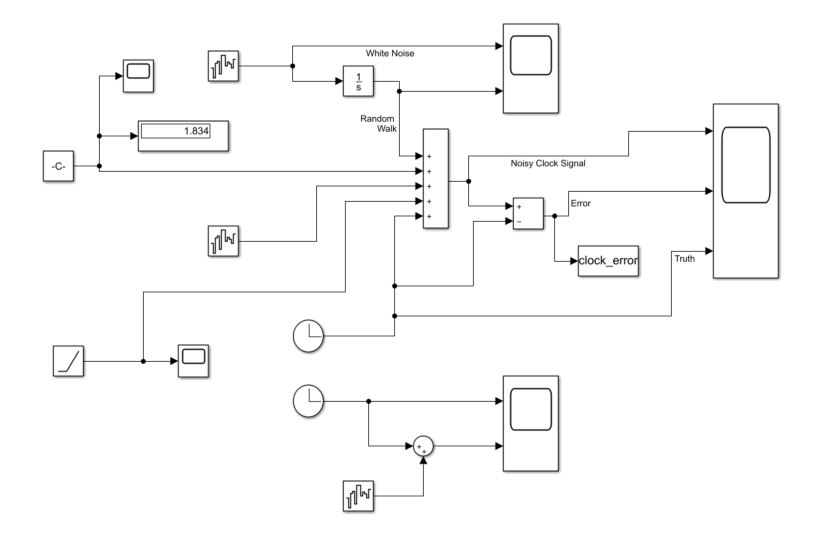
\includegraphics[scale=0.75]{day1_seg4_state_space/clock_block_diagram_model.jpg}
\onslide<1->{\center --------------------------------------------------------------------}
\end{frame}

%\begin{frame}
%missing graphic %sample_bd_01.latex
%\input{day1_seg4_state_space/sample_bd_01.latex}
\onslide<1->{\center --------------------------------------------------------------------}
%\end{frame}

% day1_seg3_state_space/deriving_state.tex
\begin{frame}
\onslide<1->{
\frametitle{Graphical Representations:  Block Diagrams}
\framesubtitle{Deriving State Equations from Block Diagrams}
}
 \begin{itemize}
 \onslide<2->{\item Continuous states can be identified as outputs of integrators
}
 \begin{itemize}
	\onslide<3->{\item First derive differential equations
}
     \onslide<4->{\item Then apply companion matrix approach to identify state dynamics matrix $A$
}
 \end{itemize}
 \onslide<5->{\item Discrete states can be identified either as sampled continous states or as outputs of delayors
}
\end{itemize}
\onslide<6->{\center --------------------------------------------------------------------}
\end{frame}

% day1_seg2_equations/examples.tex
\begin{frame}
\onslide<1->{\frametitle{Examples}
}
 \begin{itemize}
 \onslide<2->{\item Scalar Constant Dynamics
}
\onslide<3->{\item Scalar Constant Dynamics with Recursive Estimator
}
 \onslide<4->{\item Scalar Ramp Dynamics with Recursive Estimator
 \item Damped Harmonic Oscillator 
}
\end{itemize}
\onslide<5->{\center --------------------------------------------------------------------}
\end{frame}

\begin{frame}
 \onslide<1->{\frametitle{ Scalar Constant Dynamics}
}
 \begin{itemize}
 \onslide<2->{\item MATLAB/Simulink Model
}
 \onslide<3->{\item Very Simple
}
 \onslide<4->{\item Additive Noise
}
 \onslide<5->{\item No feedback loops
}
\end{itemize}
\onslide<6->{\center --------------------------------------------------------------------}
\end{frame}

\begin{frame}
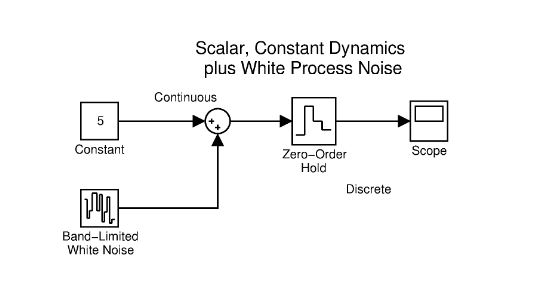
\includegraphics[scale=0.80]{matlab/scalar_const_noise.jpg}
\onslide<1->{\center --------------------------------------------------------------------}
\end{frame}

\begin{frame}
  \onslide<1->{\frametitle{Scalar Constant Dynamics with Recursive Estimator}
}
 \begin{itemize}
 \onslide<2->{\item MATLAB/Simulink Model
}
\onslide<3->{ \item Very Simple Dynamics
}
\onslide<4->{ \item Additive Noise
}
 \onslide<5->{\item Estimation loop implementing recursive simple averaging
}
 \onslide<6->{\item Simple open loop gain input
}
\end{itemize}
\onslide<7->{\center --------------------------------------------------------------------}
\end{frame}

\begin{frame}
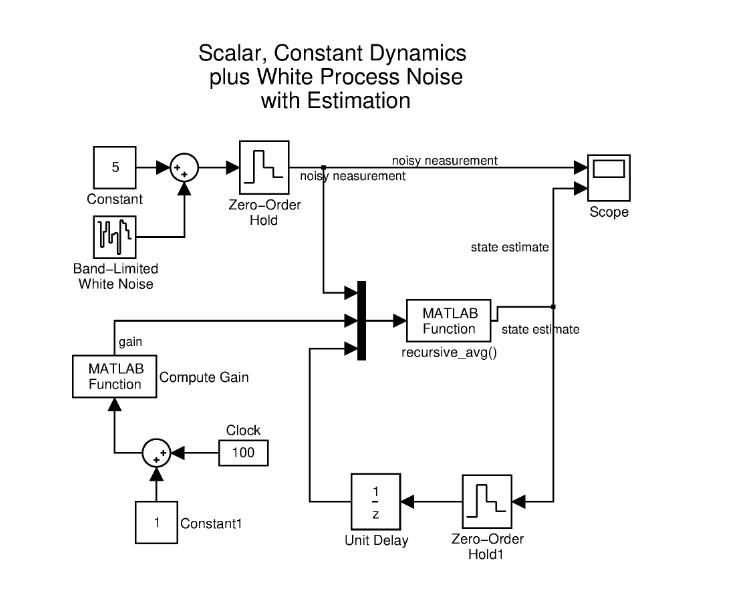
\includegraphics[scale=0.80]{day1_seg4_state_space/scalar_const_est.jpg}
\onslide<1->{\center --------------------------------------------------------------------}
\end{frame}

\begin{frame}
  \onslide<1->{\frametitle{Scalar Ramp Dynamics with Recursive Estimator}
}
 \begin{itemize}
 \onslide<2->{\item MATLAB/Simulink Model
}
 \onslide<3->{\item Scalar Dynamics with known ramp
}
 \onslide<4->{\item Additive Noise
}
 \onslide<5->{\item Estimation loop implementing recursive simple averaging
}
 \onslide<6->{\item Simple open loop gain input
}
\end{itemize}
\onslide<7->{\center --------------------------------------------------------------------}
\end{frame}

\begin{frame}
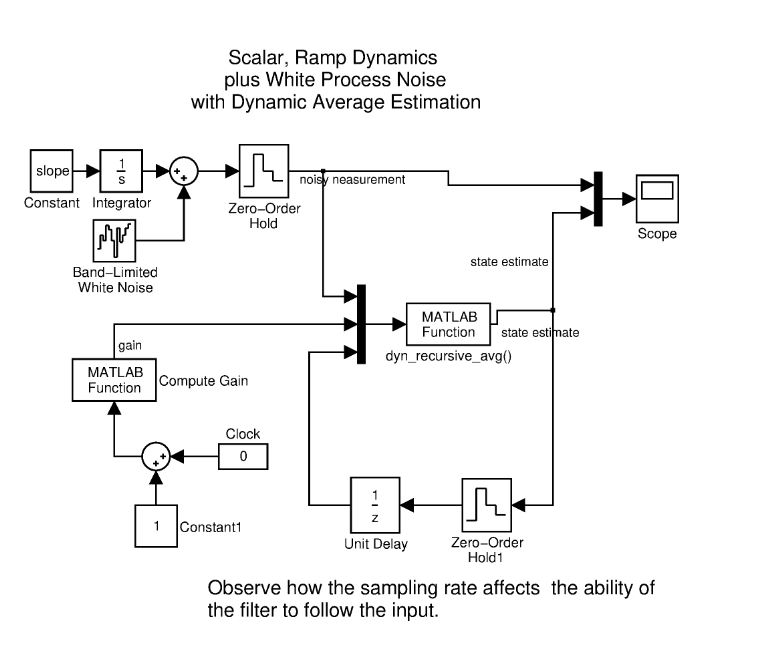
\includegraphics[scale=0.80]{matlab/scalar_ramp_noise_est.jpg}
\onslide<1->{\center --------------------------------------------------------------------}
\end{frame}

\begin{frame}
  \onslide<1->{\frametitle{Vector Dynamics: Damped Harmonic Oscillator}
}
 \begin{itemize}
 \onslide<2->{\item MATLAB/Simulink Model
}
 \onslide<3->{\item 2-dimensional Vector Dynamics
}
 \onslide<4->{\item Deterministic, Continuous Model
}
\onslide<5->{
\[
\begin{bmatrix}
\dot{x}_1\\
\dot{x}_2
\end{bmatrix} =
\begin{bmatrix}
0 & 1\\
-k/m & -c/m
\end{bmatrix}
\begin{bmatrix}
x_1\\
x_2
\end{bmatrix}
\]
}
\end{itemize}
\onslide<6->{\center --------------------------------------------------------------------}
\end{frame}

\begin{frame}
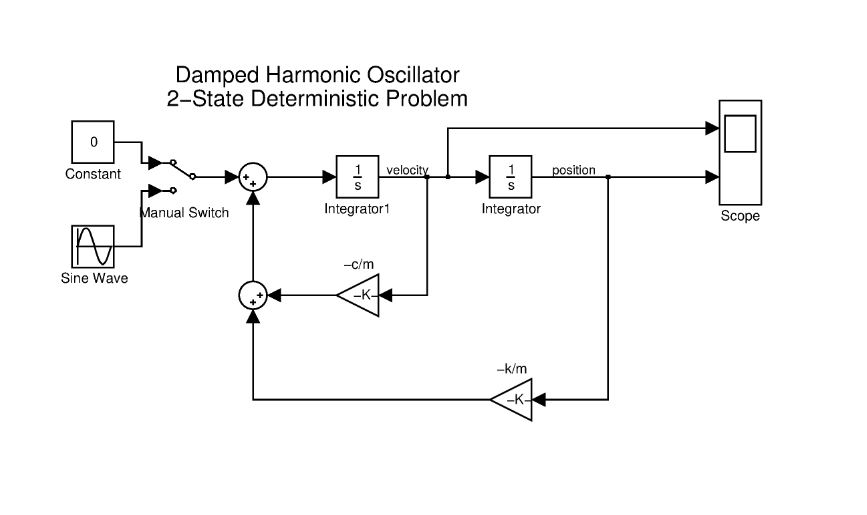
\includegraphics[scale=0.80]{day1_seg4_state_space/damped_harmosc_det.jpg}
\onslide<1->{\center --------------------------------------------------------------------}
\end{frame}

\begin{frame}
  \onslide<1->{\frametitle{Vector Dynamics: Damped Harmonic Oscillator}
}
 \begin{itemize}
 \onslide<2->{\item Discrete model would look like this}
\onslide<3->{ 
\[\begin{bmatrix}
x_{1}(k)\\
x_{2}(k)
\end{bmatrix}=\exp
\left(
\begin{bmatrix}
0 & 1\\
-k/m & -c/m
\end{bmatrix}
\Delta t
\right)
\begin{bmatrix}
x_{1}(k-1)\\
x_{2}(k-1)
\end{bmatrix}
\]
}
\onslide<3->{\item Here $\Delta t=t_k - t_{k-1}$
}
\onslide<4->{\item Note that $\exp$ is a matrix exponential
}
\onslide<5->{\item In the continuous case, the state transition matrix is a matrix exponential whenever the system dynamics matrix is a constant (i.e., time invariant) matrix
}
\end{itemize}
\onslide<6->{\center --------------------------------------------------------------------}
\end{frame}

% day1_seg3_state_space/stm.tex
\begin{frame}
\onslide<1->{\frametitle{State Transition Matrix}
}
\begin{itemize}
\onslide<2->{ 
	\item $\Phi(t,t_0)$
}
\onslide<3->{ 
	\item Needed when deriving a discrete-time state space model from a continuous-time model
 }
\onslide<4->{ 
	\item Solution of homogeneous (zero-input) equation for continuous-time systems
 }
\onslide<5->{
	\item If discrete-time system is derived from continuous-time system, then $\stmeq{k}$ satisfies:
\[
x_k=\stm{k}x_{k-1}
\]}
\end{itemize}
\onslide<6->{\center --------------------------------------------------------------------}
\end{frame}

\begin{frame}
\onslide<1->{
\frametitle{State Transition Matrix}
}
\begin{itemize}
\onslide<2->{ 
	\item $\Phi$ satisfies matrix differential equation:  $\dot{\Phi}(t,t_0)=A(t)\Phi(t,t_0)$\\
	with initial condition:  $\Phi(t_0,t_0)=I$
}
\onslide<3->{ 
	\item For a time-invariant system ($A$ is constant):  $\dot{x}(t)=Ax(t)$, solution is $\Phi(t_2,t_1)=\exp(A(t_2-t_1))$\\
}
\onslide<4->{ 
	\item For a time-varying system:  $\dot{x}(t)=A(t)x(t)$, there is NO general solution. \\
	But solutions can be found in special circumstances and several series solutions 
	are available.\\
	E.g., 	If $A(t)A(s)=A(s)A(t)$ for every pair of times $t,s$, then $\Phi(t_2,t_1)=\exp\left(\int_{t_1}^{t_2}A(\tau)d\tau\right)$

}
\end{itemize}
\onslide<5->{\center --------------------------------------------------------------------}
\end{frame}

\begin{frame}
  \onslide<1->{
	\frametitle{State Transition Matrix} 
	\framesubtitle{Properties of $\Phi$}
}
\begin{itemize}
  \onslide<2->{
\item  Transition Property: $\Phi(t_3,t_1)=\Phi(t_3,t_2)\Phi(t_2,t_1)$
}
  \onslide<3->{
\item  Inversion Property:  $\Phi^{-1}(t_2,t_1)=\Phi(t_1,t_2)$ 
}
  \onslide<4->{
	\item Separation Property:  $\Phi$ can be written as $\Phi(t_2,t_1)=\theta(t_2)\theta^{-1}(t_1)$, where $\theta$ is the solution to the matrix differential equation:\\
$\dot{\theta}(t)=A(t)\theta(t)$
}
  \onslide<5->{
	\item Determinant Property:  $\det{\Phi(t_2,t_1)}=\exp\left(\int_{t_1}^{t_2}\trace{A(\tau)}d\tau\right)$
}
\end{itemize}
\onslide<6->{\center --------------------------------------------------------------------}
\end{frame}

\begin{frame}
  \onslide<1->{
	\frametitle{State Transition Matrix} 
	\framesubtitle{Solving for $\Phi$}
}
\begin{itemize}
  \onslide<2->{
\item  Peano-Baker Series (valid even for time-varying $A(t)$):\\
$\Phi(t_2,t_1)=I+\int_{t_1}^{t_2}A(s_1)ds_1+\int_{t_1}^{t_2}A(s_1)\int_{t_1}^{s_1}A(s_2)ds_2ds_1+\cdots$
}
  \onslide<3->{
\item Another series solution is given by the Magnus series expansion involving matrix commutators  
\begin{itemize}
\item Truncated Magnus expansions exhibit many of the properties of $\Phi$
\end{itemize}
}
\end{itemize}
\onslide<4->{\center --------------------------------------------------------------------}
\end{frame}
\begin{frame}
  \onslide<1->{
	\frametitle{State Transition Matrix} 
	\framesubtitle{MATLAB Symbolic Toolbox}
}
  \onslide<2->{

syms dt;  n=8; A = zeros(n); A(1:n-1,2:n)=eye(n-1); expm(A*dt)\\
}
  \onslide<3->{
  \begin{footnotesize}
    $\Phi(t_k,t_{k-1})=\left(\begin{array}{cccccccc} 1 & \mathrm{dt} & \frac{{\mathrm{dt}}^2}{2} & \frac{{\mathrm{dt}}^3}{6} & \frac{{\mathrm{dt}}^4}{24} & \frac{{\mathrm{dt}}^5}{120} & \frac{{\mathrm{dt}}^6}{720} & \frac{{\mathrm{dt}}^7}{5040}\\ 0 & 1 & \mathrm{dt} & \frac{{\mathrm{dt}}^2}{2} & \frac{{\mathrm{dt}}^3}{6} & \frac{{\mathrm{dt}}^4}{24} & \frac{{\mathrm{dt}}^5}{120} & \frac{{\mathrm{dt}}^6}{720}\\ 0 & 0 & 1 & \mathrm{dt} & \frac{{\mathrm{dt}}^2}{2} & \frac{{\mathrm{dt}}^3}{6} & \frac{{\mathrm{dt}}^4}{24} & \frac{{\mathrm{dt}}^5}{120}\\ 0 & 0 & 0 & 1 & \mathrm{dt} & \frac{{\mathrm{dt}}^2}{2} & \frac{{\mathrm{dt}}^3}{6} & \frac{{\mathrm{dt}}^4}{24}\\ 0 & 0 & 0 & 0 & 1 & \mathrm{dt} & \frac{{\mathrm{dt}}^2}{2} & \frac{{\mathrm{dt}}^3}{6}\\ 0 & 0 & 0 & 0 & 0 & 1 & \mathrm{dt} & \frac{{\mathrm{dt}}^2}{2}\\ 0 & 0 & 0 & 0 & 0 & 0 & 1 & \mathrm{dt}\\ 0 & 0 & 0 & 0 & 0 & 0 & 0 & 1 \end{array}\right)$\\
	where $dt=t_k-t_{k-1}$
	\end{footnotesize}

  }
\onslide<4->{\center --------------------------------------------------------------------}
\end{frame}
%\begin{frame}
%  \onslide<1->{
%	\frametitle{State Transition Matrix} 
%	\framesubtitle{MATLAB Symbolic Toolbox: Companion Matrix}
%}
%\begin{tiny}
%  \onslide<2->{
%For $\left(\begin{array}{cc} 0 & 1\\ -a_{0} & -a_{1} \end{array}\right)$ 
%}
%  \onslide<3->{
%$\Phi_{11}=\frac{{\mathrm{e}}^{-\frac{\mathrm{dt}\,\sqrt{{a_{1}}^2-4\,a_{0}}}{2}-\frac{a_{1}\,\mathrm{dt}}{2}}\,\sqrt{{a_{1}}^2-4\,a_{0}}+{\mathrm{e}}^{\frac{\mathrm{dt}\,\sqrt{{a_{1}}^2-4\,a_{0}}}{2}-\frac{a_{1}\,\mathrm{dt}}{2}}\,\sqrt{{a_{1}}^2-4\,a_{0}}-a_{1}\,{\mathrm{e}}^{-\frac{\mathrm{dt}\,\sqrt{{a_{1}}^2-4\,a_{0}}}{2}-\frac{a_{1}\,\mathrm{dt}}{2}}+a_{1}\,{\mathrm{e}}^{\frac{\mathrm{dt}\,\sqrt{{a_{1}}^2-4\,a_{0}}}{2}-\frac{a_{1}\,\mathrm{dt}}{2}}}{2\,\sqrt{{a_{1}}^2-4\,a_{0}}}'$
%}
%\end{tiny}
\onslide<4->{\center --------------------------------------------------------------------}
%\end{frame}

% day1_seg3_state_space/exercises.tex
\begin{frame}
Exercises
 \begin{enumerate}
 \item Convert the differential equation
\[5\frac{d^3y}{dt^3}-0.3\frac{dy}{dt}+7y=u(t)\]
into a state space system model
 \item Convert the difference equation
\[100y(k+9) = \sum_{i=0}^2b_iu(k+2-i)\]
 \item Write the output equations for the above systems as well!
\end{enumerate}
\onslide<1->{\center --------------------------------------------------------------------}
\end{frame}


% ----------------------------------------------------------------
\end{document}
